    \documentclass[dvipsnames]{beamer}
    \usetheme{Madrid}
    \usefonttheme{professionalfonts}
    \usepackage{
        amsmath,
        amssymb,
        fouriernc, % fourier font w/ new century book
        fancyhdr, % page styling
        lastpage, % footer fanciness
        hyperref, % various links
        setspace, % line spacing
        amsthm, % newtheorem and proof environment
        mathtools, % \Aboxed for boxing inside aligns, among others
        float, % Allow [H] figure env alignment
        enumerate, % Allow custom enumerate numbering
        graphicx, % allow includegraphics with more filetypes
        wasysym, % \smiley!
        upgreek, % \upmu for \mum macro
        listings, % writing TrueType fonts and including code prettily
        tikz, % drawing things
        booktabs, % \bottomrule instead of hline apparently
        cancel % can cancel things out!
    }
    \usepackage[
        labelfont=bf, % caption names are labeled in bold
        font=scriptsize % smaller font for captions
    ]{caption}
    \usepackage[font=scriptsize]{subcaption} % subfigures

    \newcommand*{\scinot}[2]{#1\times10^{#2}}
    \newcommand*{\dotp}[2]{\left<#1\,\middle|\,#2\right>}
    \newcommand*{\rd}[2]{\frac{\mathrm{d}#1}{\mathrm{d}#2}}
    \newcommand*{\pd}[2]{\frac{\partial#1}{\partial#2}}
    \newcommand*{\rtd}[2]{\frac{\mathrm{d}^2#1}{\mathrm{d}#2^2}}
    \newcommand*{\ptd}[2]{\frac{\partial^2 #1}{\partial#2^2}}
    \newcommand*{\md}[2]{\frac{\mathrm{D}#1}{\mathrm{D}#2}}
    \newcommand*{\pvec}[1]{\vec{#1}^{\,\prime}}
    \newcommand*{\svec}[1]{\vec{#1}\;\!}
    \newcommand*{\bm}[1]{\boldsymbol{\mathbf{#1}}}
    \newcommand*{\ang}[0]{\;\text{\AA}}
    \newcommand*{\mum}[0]{\;\upmu \mathrm{m}}
    \newcommand*{\at}[1]{\left.#1\right|}

    \let\Re\undefined
    \let\Im\undefined
    \DeclareMathOperator{\Res}{Res}
    \DeclareMathOperator{\Re}{Re}
    \DeclareMathOperator{\Im}{Im}
    \DeclareMathOperator{\Log}{Log}
    \DeclareMathOperator{\Arg}{Arg}
    \DeclareMathOperator{\Tr}{Tr}
    \DeclareMathOperator{\E}{E}
    \DeclareMathOperator{\Var}{Var}
    \DeclareMathOperator*{\argmin}{argmin}
    \DeclareMathOperator*{\argmax}{argmax}
    \DeclareMathOperator{\sgn}{sgn}
    \DeclareMathOperator{\diag}{diag\;}

    \DeclarePairedDelimiter\bra{\langle}{\rvert}
    \DeclarePairedDelimiter\ket{\lvert}{\rangle}
    \DeclarePairedDelimiter\abs{\lvert}{\rvert}
    \DeclarePairedDelimiter\ev{\langle}{\rangle}
    \DeclarePairedDelimiter\p{\lparen}{\rparen}
    \DeclarePairedDelimiter\s{\lbrack}{\rbrack}
    \DeclarePairedDelimiter\z{\lbrace}{\rbrace}

    % \everymath{\displaystyle} % biggify limits of inline sums and integrals
    \tikzstyle{circ} % usage: \node[circ, placement] (label) {text};
        = [draw, circle, fill=white, node distance=3cm, minimum height=2em]
    \definecolor{commentgreen}{rgb}{0,0.6,0}
    \lstset{
        basicstyle=\ttfamily\footnotesize,
        frame=single,
        numbers=left,
        showstringspaces=false,
        keywordstyle=\color{blue},
        stringstyle=\color{purple},
        commentstyle=\color{commentgreen},
        morecomment=[l][\color{magenta}]{\#}
    }


\AtBeginSection[]
{
  \begin{frame}<beamer>
    \frametitle{Overview}
    \tableofcontents[currentsection]
  \end{frame}
}

\begin{document}

\title[Disks \& Obliquities]{Extending Planet Obliquity Excitation with a
Dissipating Protoplanetary Disk}
\subtitle{Cornell Astrophysics Lunch}
\author{Yubo Su}
\date{Oct 02, 2019}

\maketitle

\section{Introduction}

\begin{frame}
    \frametitle{Introduction}
    \framesubtitle{High Obliquity Exoplanets and Secular Spin-Orbit Resonances}

    \begin{figure}[t]
        \centering
        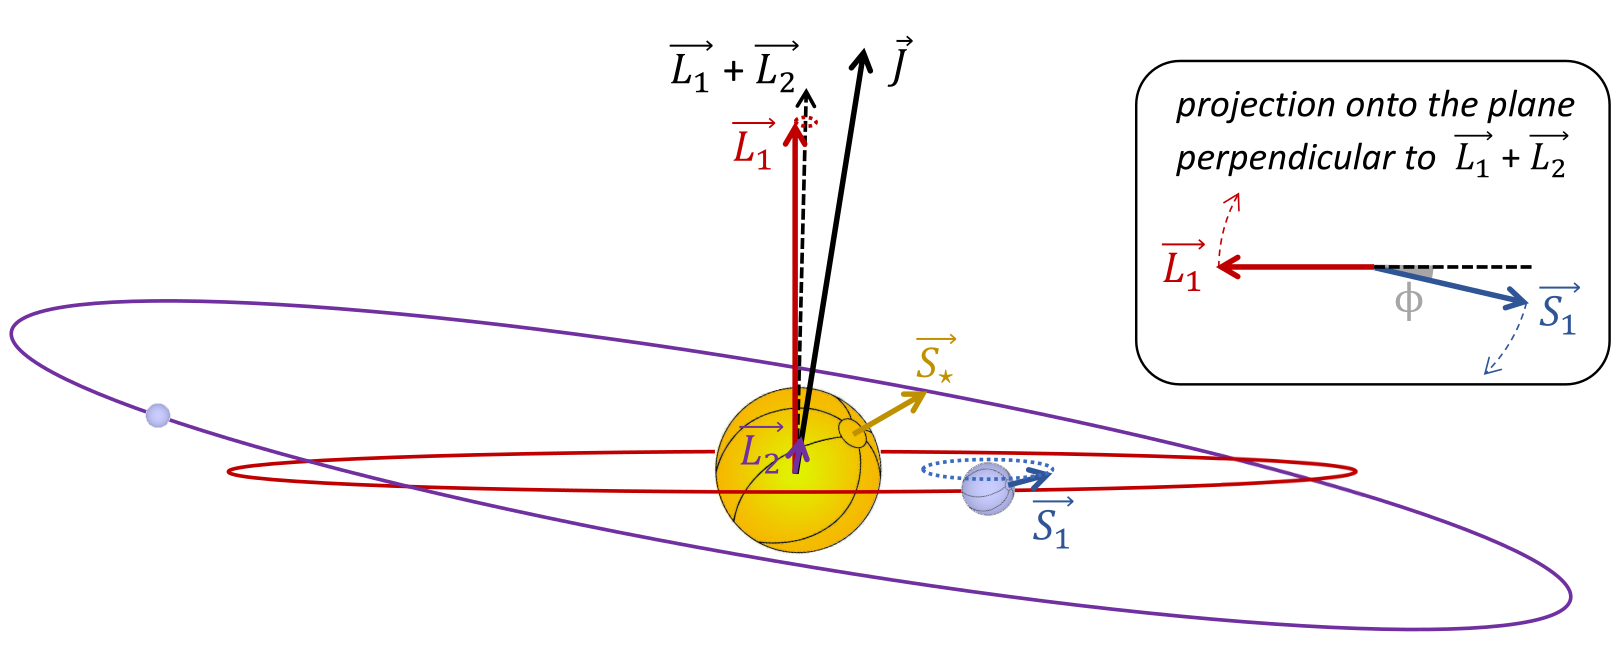
\includegraphics[width=0.7\textwidth]{millholland_laughlin.png}
        \caption{Millholland \& Laughlin 2018.}
    \end{figure}
    \begin{columns}
        \begin{column}{0.5\textwidth}
            \begin{itemize}
                \item Planet obliquity $\theta = \cos^{-1}\p*{\hat{S}_1 \cdot
                    \hat{L}_1}$.
                \item Obliquity tides.
                \item Atmospheric circulation.
            \end{itemize}
        \end{column}
        \begin{column}{0.5\textwidth}
            \begin{itemize}
                \item Probe unseen companions.
                \item Active in Saturn ($26^\circ.7$) \& Neptune.
            \end{itemize}
        \end{column}
    \end{columns}
\end{frame}

\begin{frame}
    \frametitle{Introduction}
    \framesubtitle{Equations}

    \begin{columns}
        \begin{column}{0.5\textwidth}
            \begin{figure}[t]
                \centering
                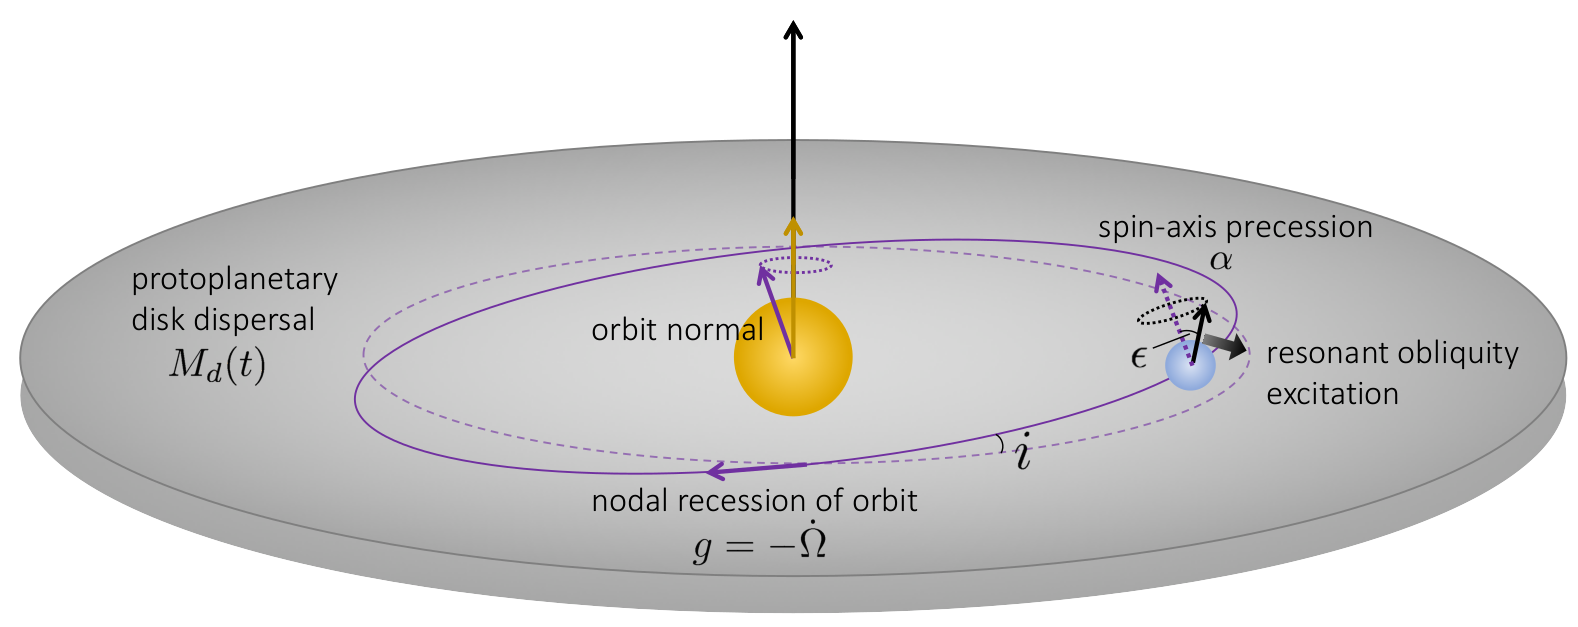
\includegraphics[width=\textwidth]{../GM_190913/1millholland_disk.png}
                \caption{Millholland \& Batygin, 2019.}
            \end{figure}
        \end{column}
        \begin{column}{0.5\textwidth}
            \begin{align*}
                \rd{\hat{s}}{t} &= \alpha \p*{\hat{s} \cdot \hat{l}_d}
                    \p*{\hat{s} \times \hat{l}_d},\\
                \rd{\hat{l}}{t} &= -g\p*{\hat{l} \cdot \hat{l}_d}
                    \p*{\hat{l} \times \hat{l}_d},\\
                \\
                \Rightarrow \rd{\hat{s}}{t}
                    &= \p{\hat{s} \cdot \hat{l}}
                        \p{\hat{s} \times \hat{l}}
                    - \eta\p{\hat{s} \times \hat{l}_d}.
            \end{align*}
            where $\eta \equiv \frac{g\cos I}{\alpha}$, $I =
            \cos^{-1}\p*{\hat{l}_d \cdot \hat{l}}$, $\alpha t \to t$.
        \end{column}
    \end{columns}
\end{frame}

\begin{frame}
    \frametitle{Introduction}
    \framesubtitle{Cassini States}

    \begin{columns}
        \begin{column}{0.5\textwidth}
            \begin{figure}
                \centering
                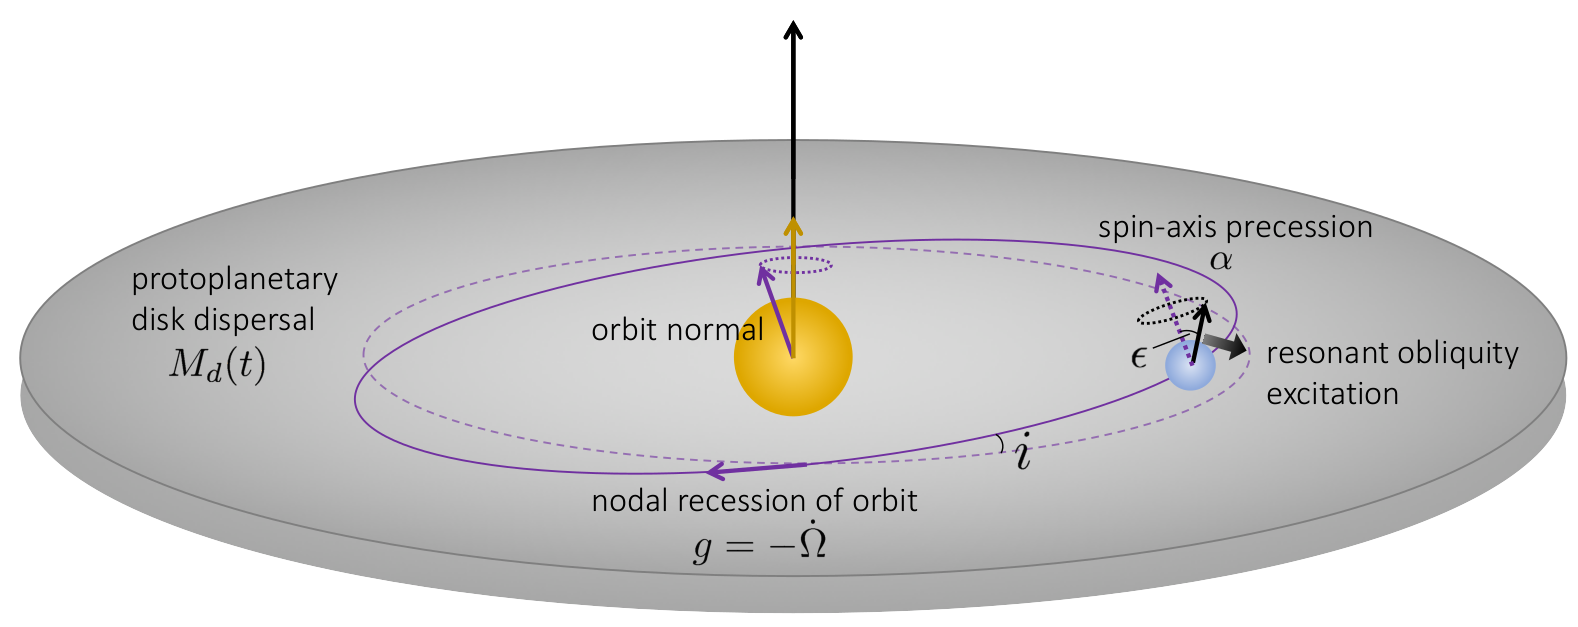
\includegraphics[width=\textwidth]{../GM_190913/1millholland_disk.png}
                \caption{Millholland \& Batygin, 2019. $\eta \equiv \frac{g\cos
                I}{\alpha}$}
            \end{figure}
            \begin{equation*}
                \rd{\hat{s}}{t}
                    = \p{\hat{s} \cdot \hat{l}}
                        \p{\hat{s} \times \hat{l}}
                    - \eta\p{\hat{s} \times \hat{l}_d}
            \end{equation*}
        \end{column}
        \begin{column}{0.5\textwidth}
            \begin{figure}
                \centering
                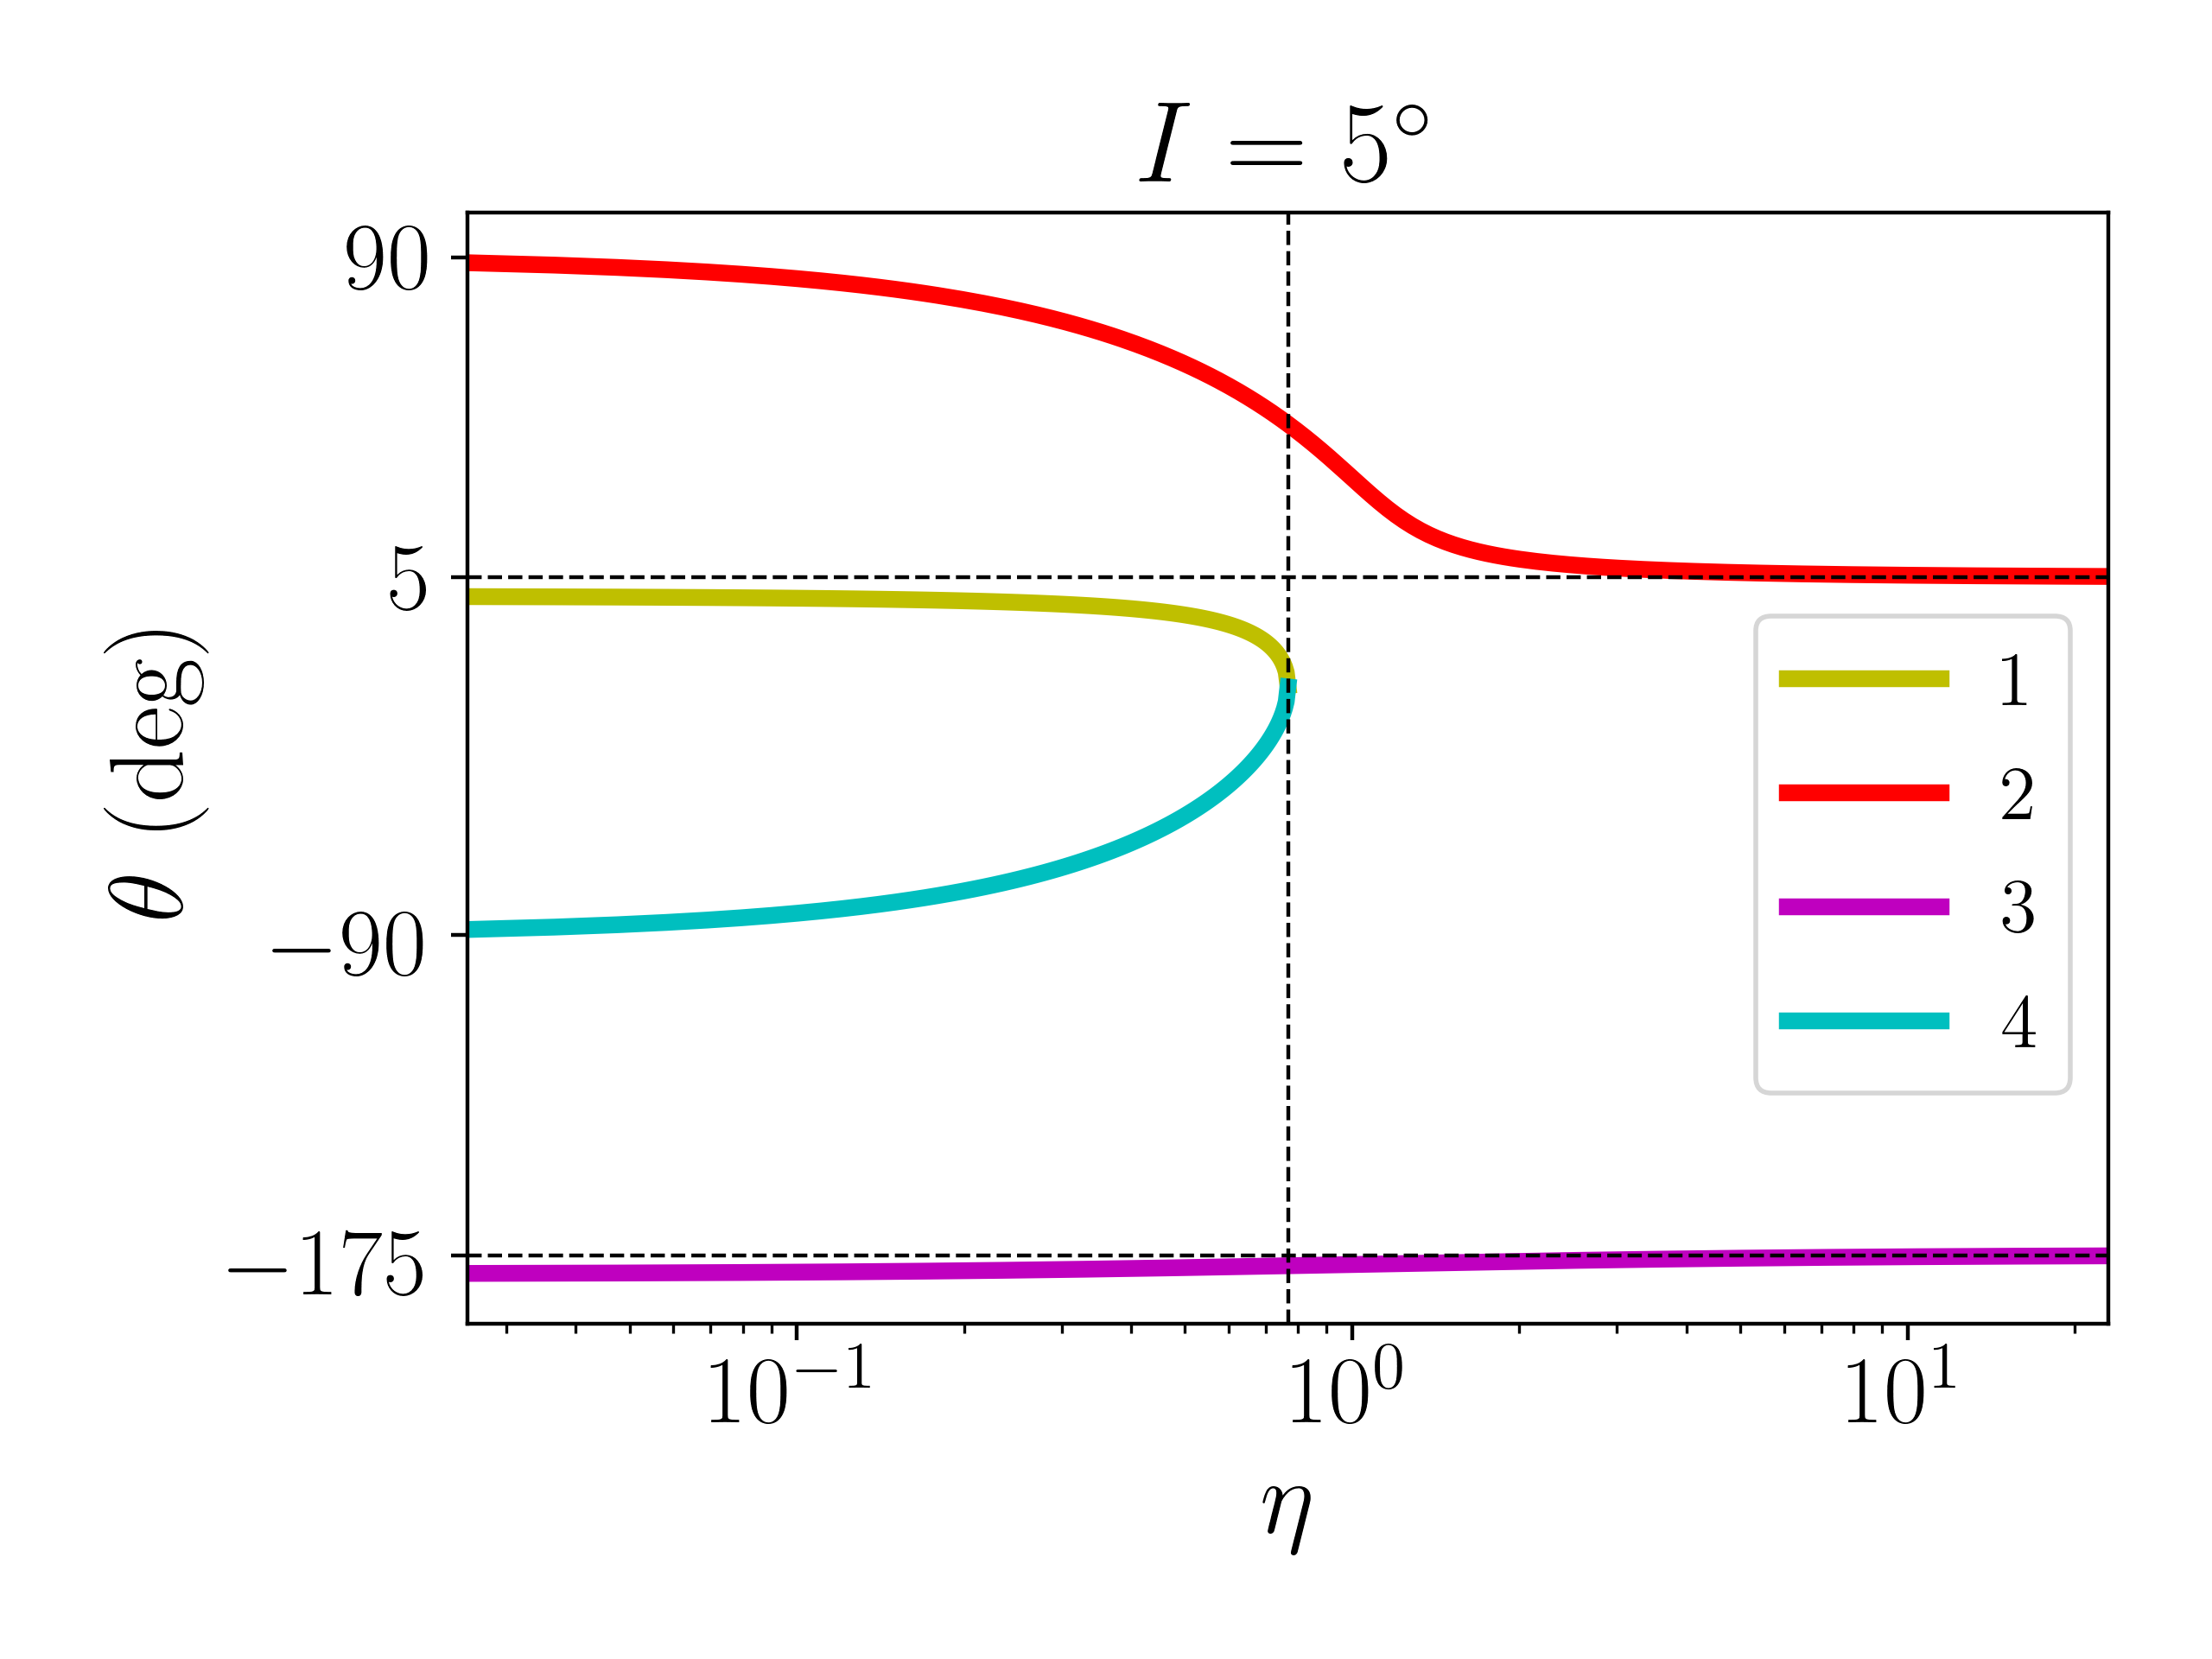
\includegraphics[width=\textwidth]{../../initial/99_misc/2_cs_locs.png}
            \end{figure}
        \end{column}
    \end{columns}
\end{frame}

\begin{frame}
    \frametitle{Introduction}
    \framesubtitle{Cassini States}

    \begin{columns}
        \begin{column}{0.5\textwidth}
            \begin{figure}
                \centering
                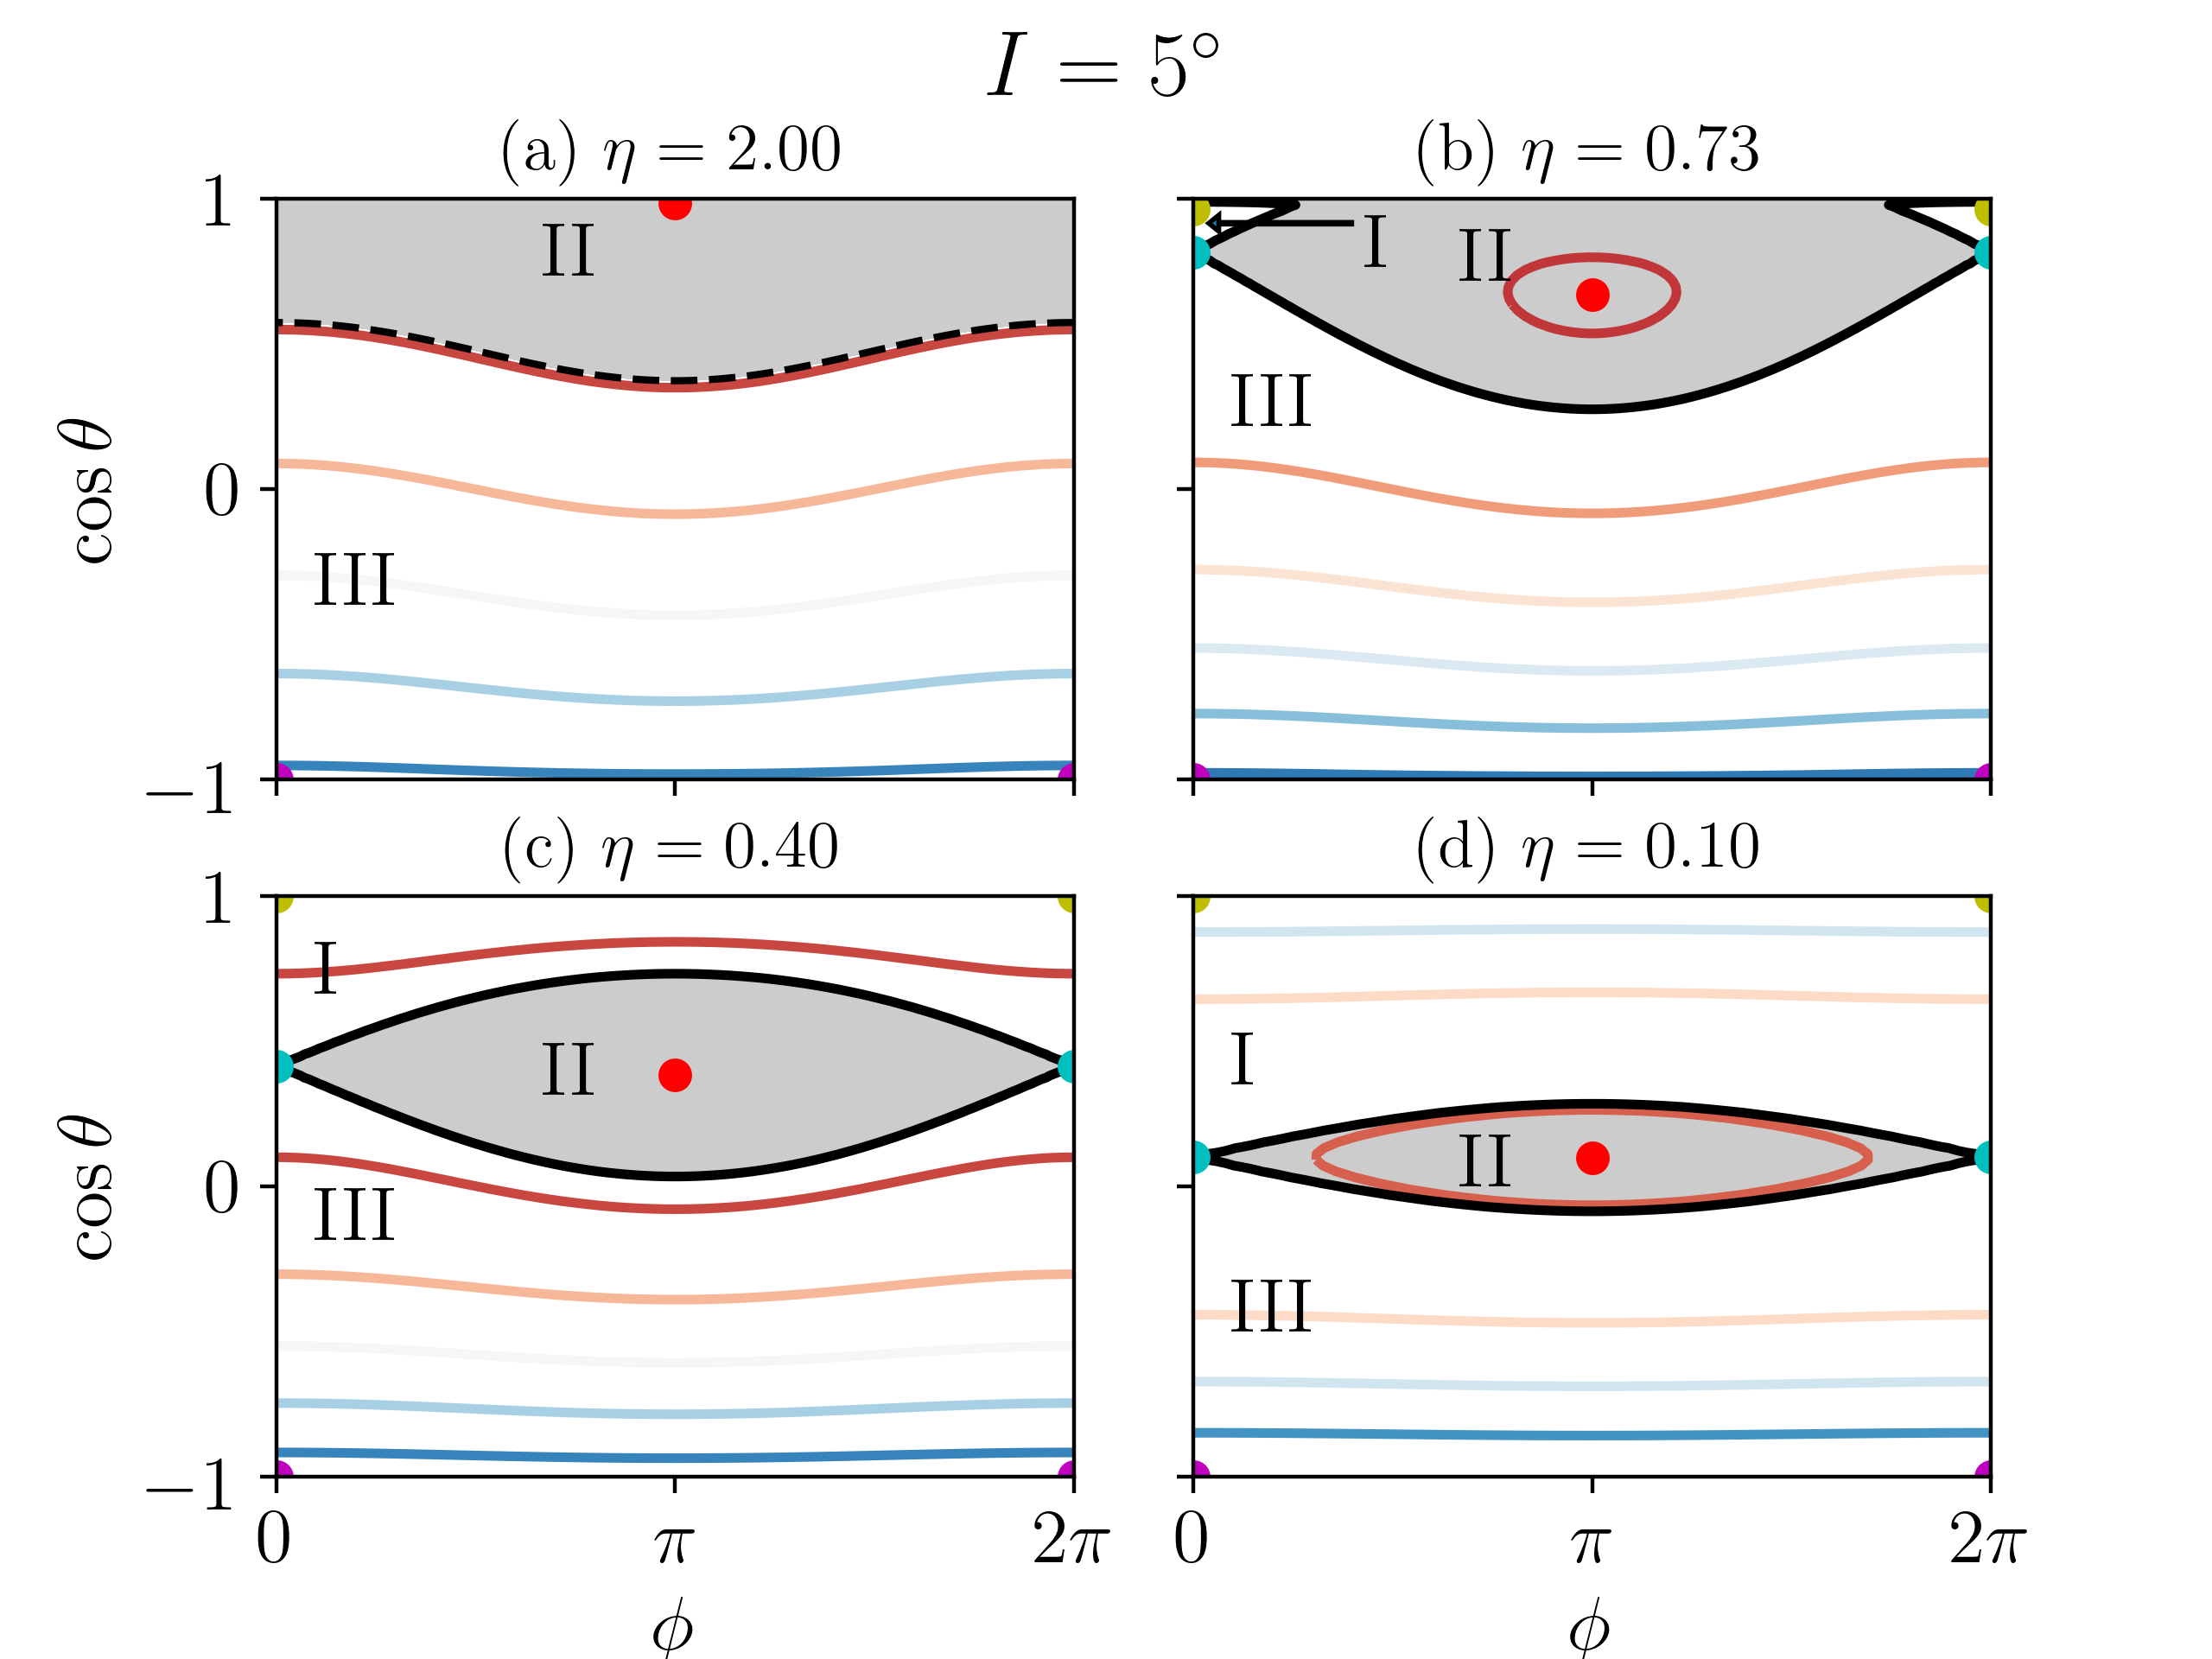
\includegraphics[width=\textwidth]{../../initial/0_eta/1contours_flip.png}
            \end{figure}
        \end{column}
        \begin{column}{0.5\textwidth}
            \begin{figure}
                \centering
                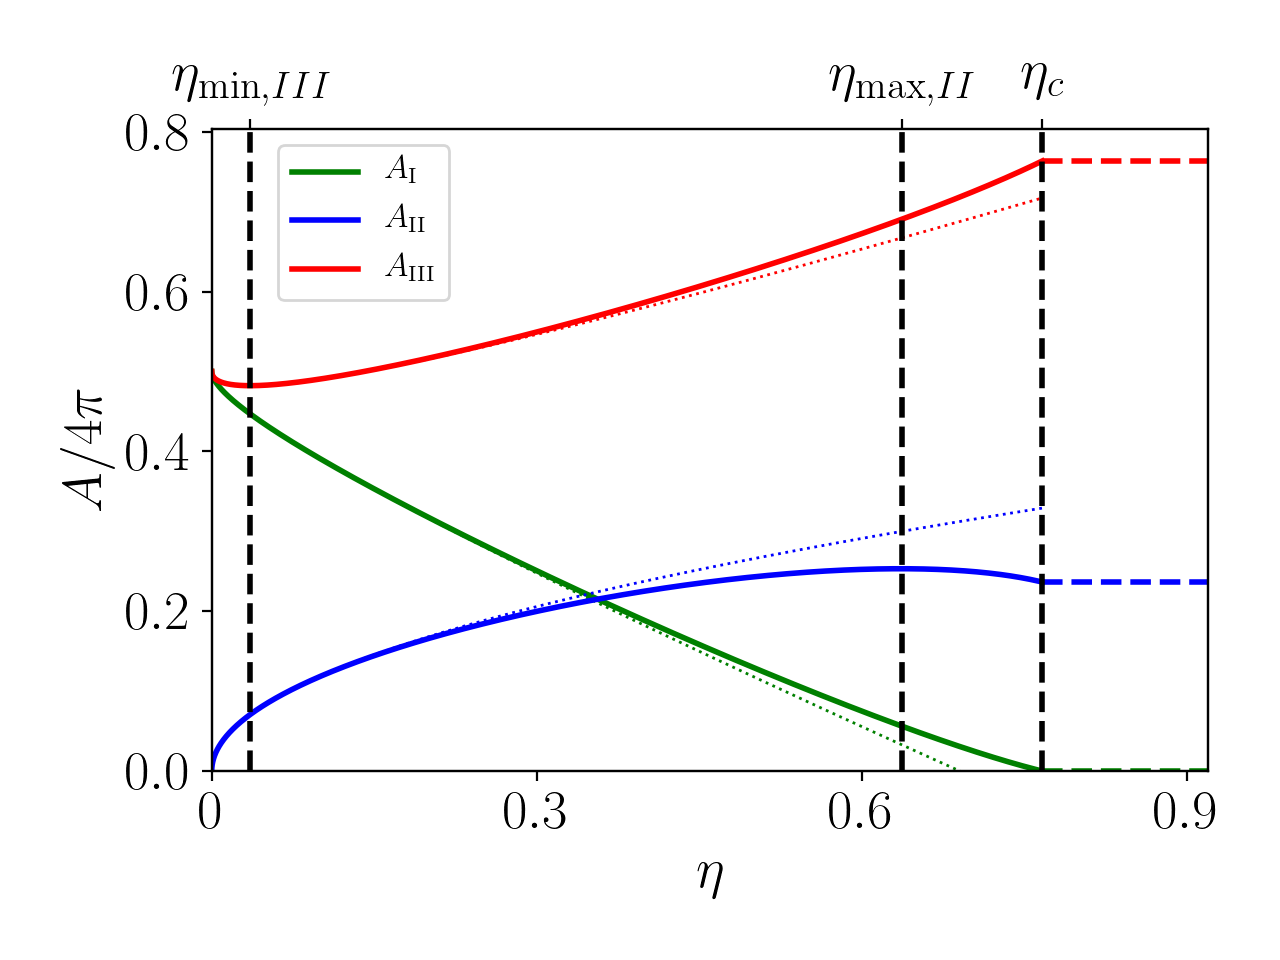
\includegraphics[width=\textwidth]{../../initial/99_misc/1_areas.png}
            \end{figure}
        \end{column}
    \end{columns}
\end{frame}

\section{Adiabatic Dynamics}

\begin{frame}
    \frametitle{Adiabatic Dynamics}
    \framesubtitle{Equations}

    \begin{columns}
        \begin{column}{0.5\textwidth}
            \begin{figure}[t]
                \centering
                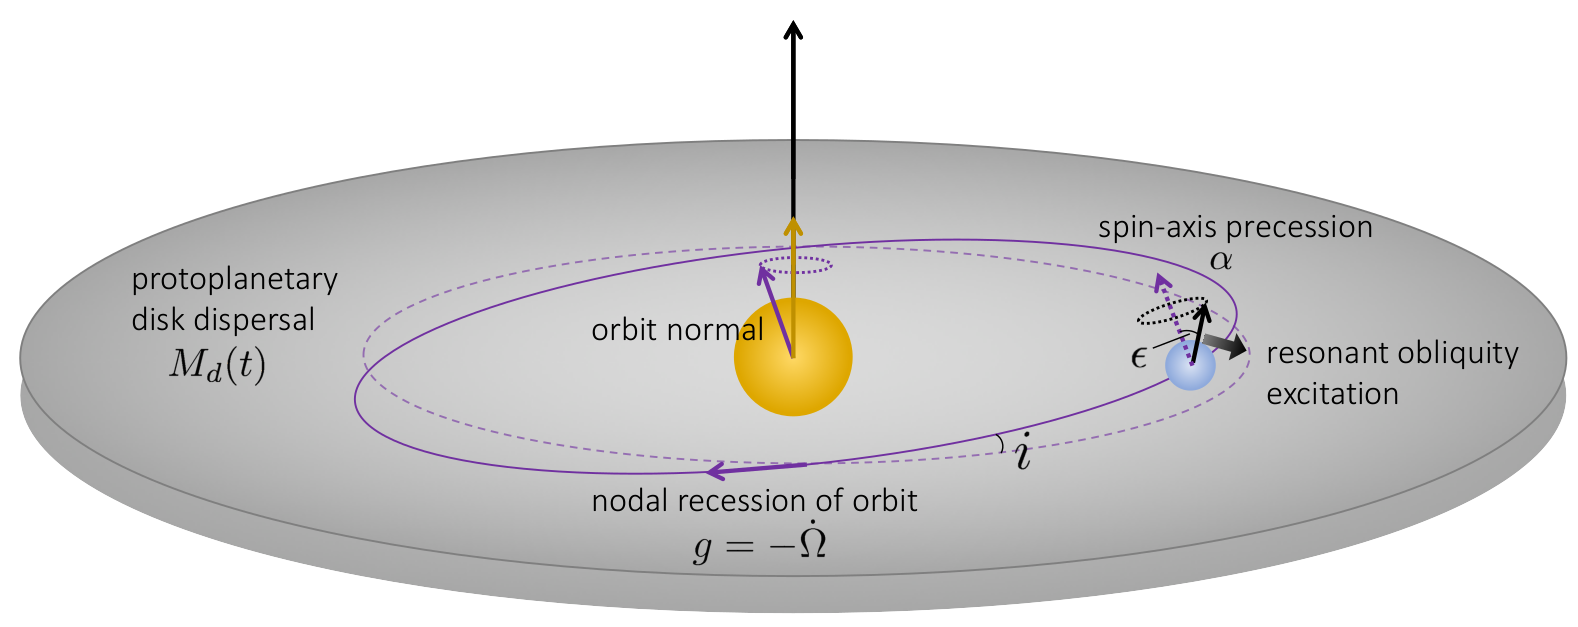
\includegraphics[width=\textwidth]{../GM_190913/1millholland_disk.png}
                \caption{Millholland \& Batygin, 2019.}
            \end{figure}
        \end{column}
        \begin{column}{0.5\textwidth}
            \begin{equation*}
                \rd{\hat{s}}{t}
                    = \p{\hat{s} \cdot \hat{l}}
                        \p{\hat{s} \times \hat{l}}
                    - \eta\p{\hat{s} \times \hat{l}_d}.
            \end{equation*}

            Let $\rd{\eta}{t} = -\epsilon \eta$, $\epsilon$ \emph{sufficiently}
            small.
        \end{column}
    \end{columns}
\end{frame}

\begin{frame}
    \frametitle{Adiabatic Dynamics}
    \framesubtitle{Adiabatic Resonance Advection}

    \begin{columns}
        \begin{column}{0.5\textwidth}
            \begin{figure}[t]
                \centering
                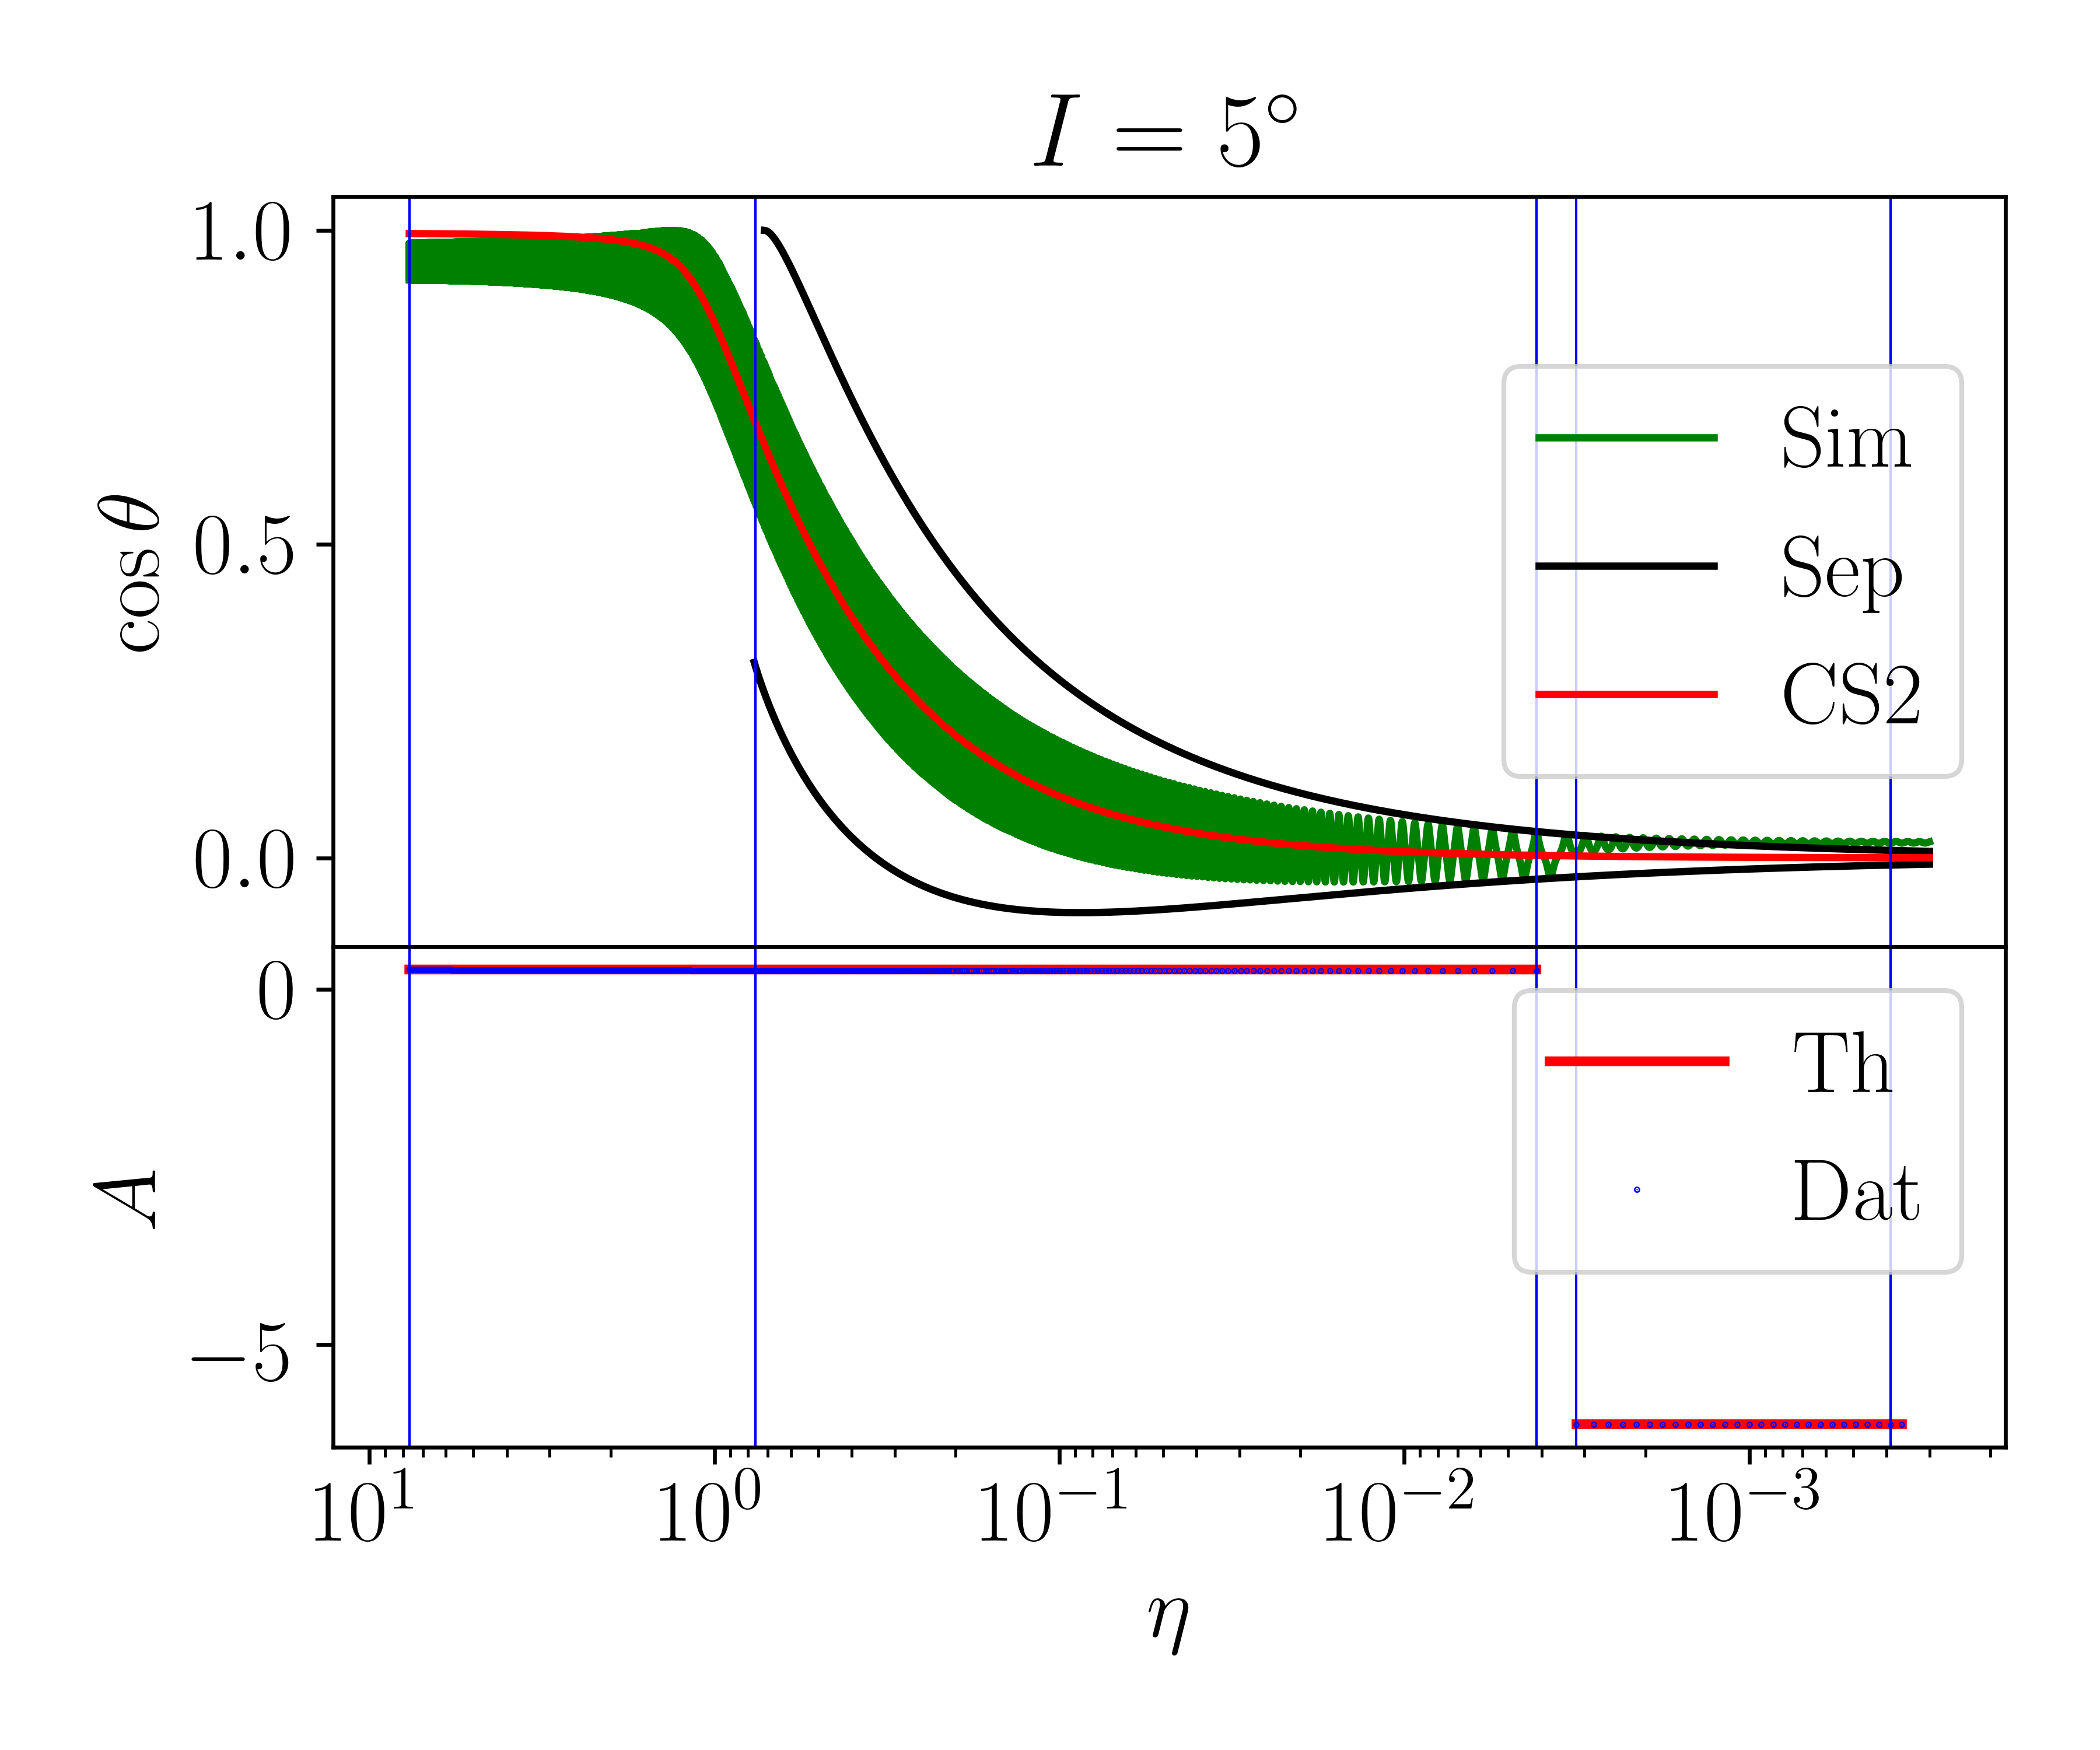
\includegraphics[width=\textwidth]{../../initial/2_toy2/3testo21.png}
            \end{figure}
        \end{column}
        \begin{column}{0.5\textwidth}
            \begin{figure}[t]
                \centering
                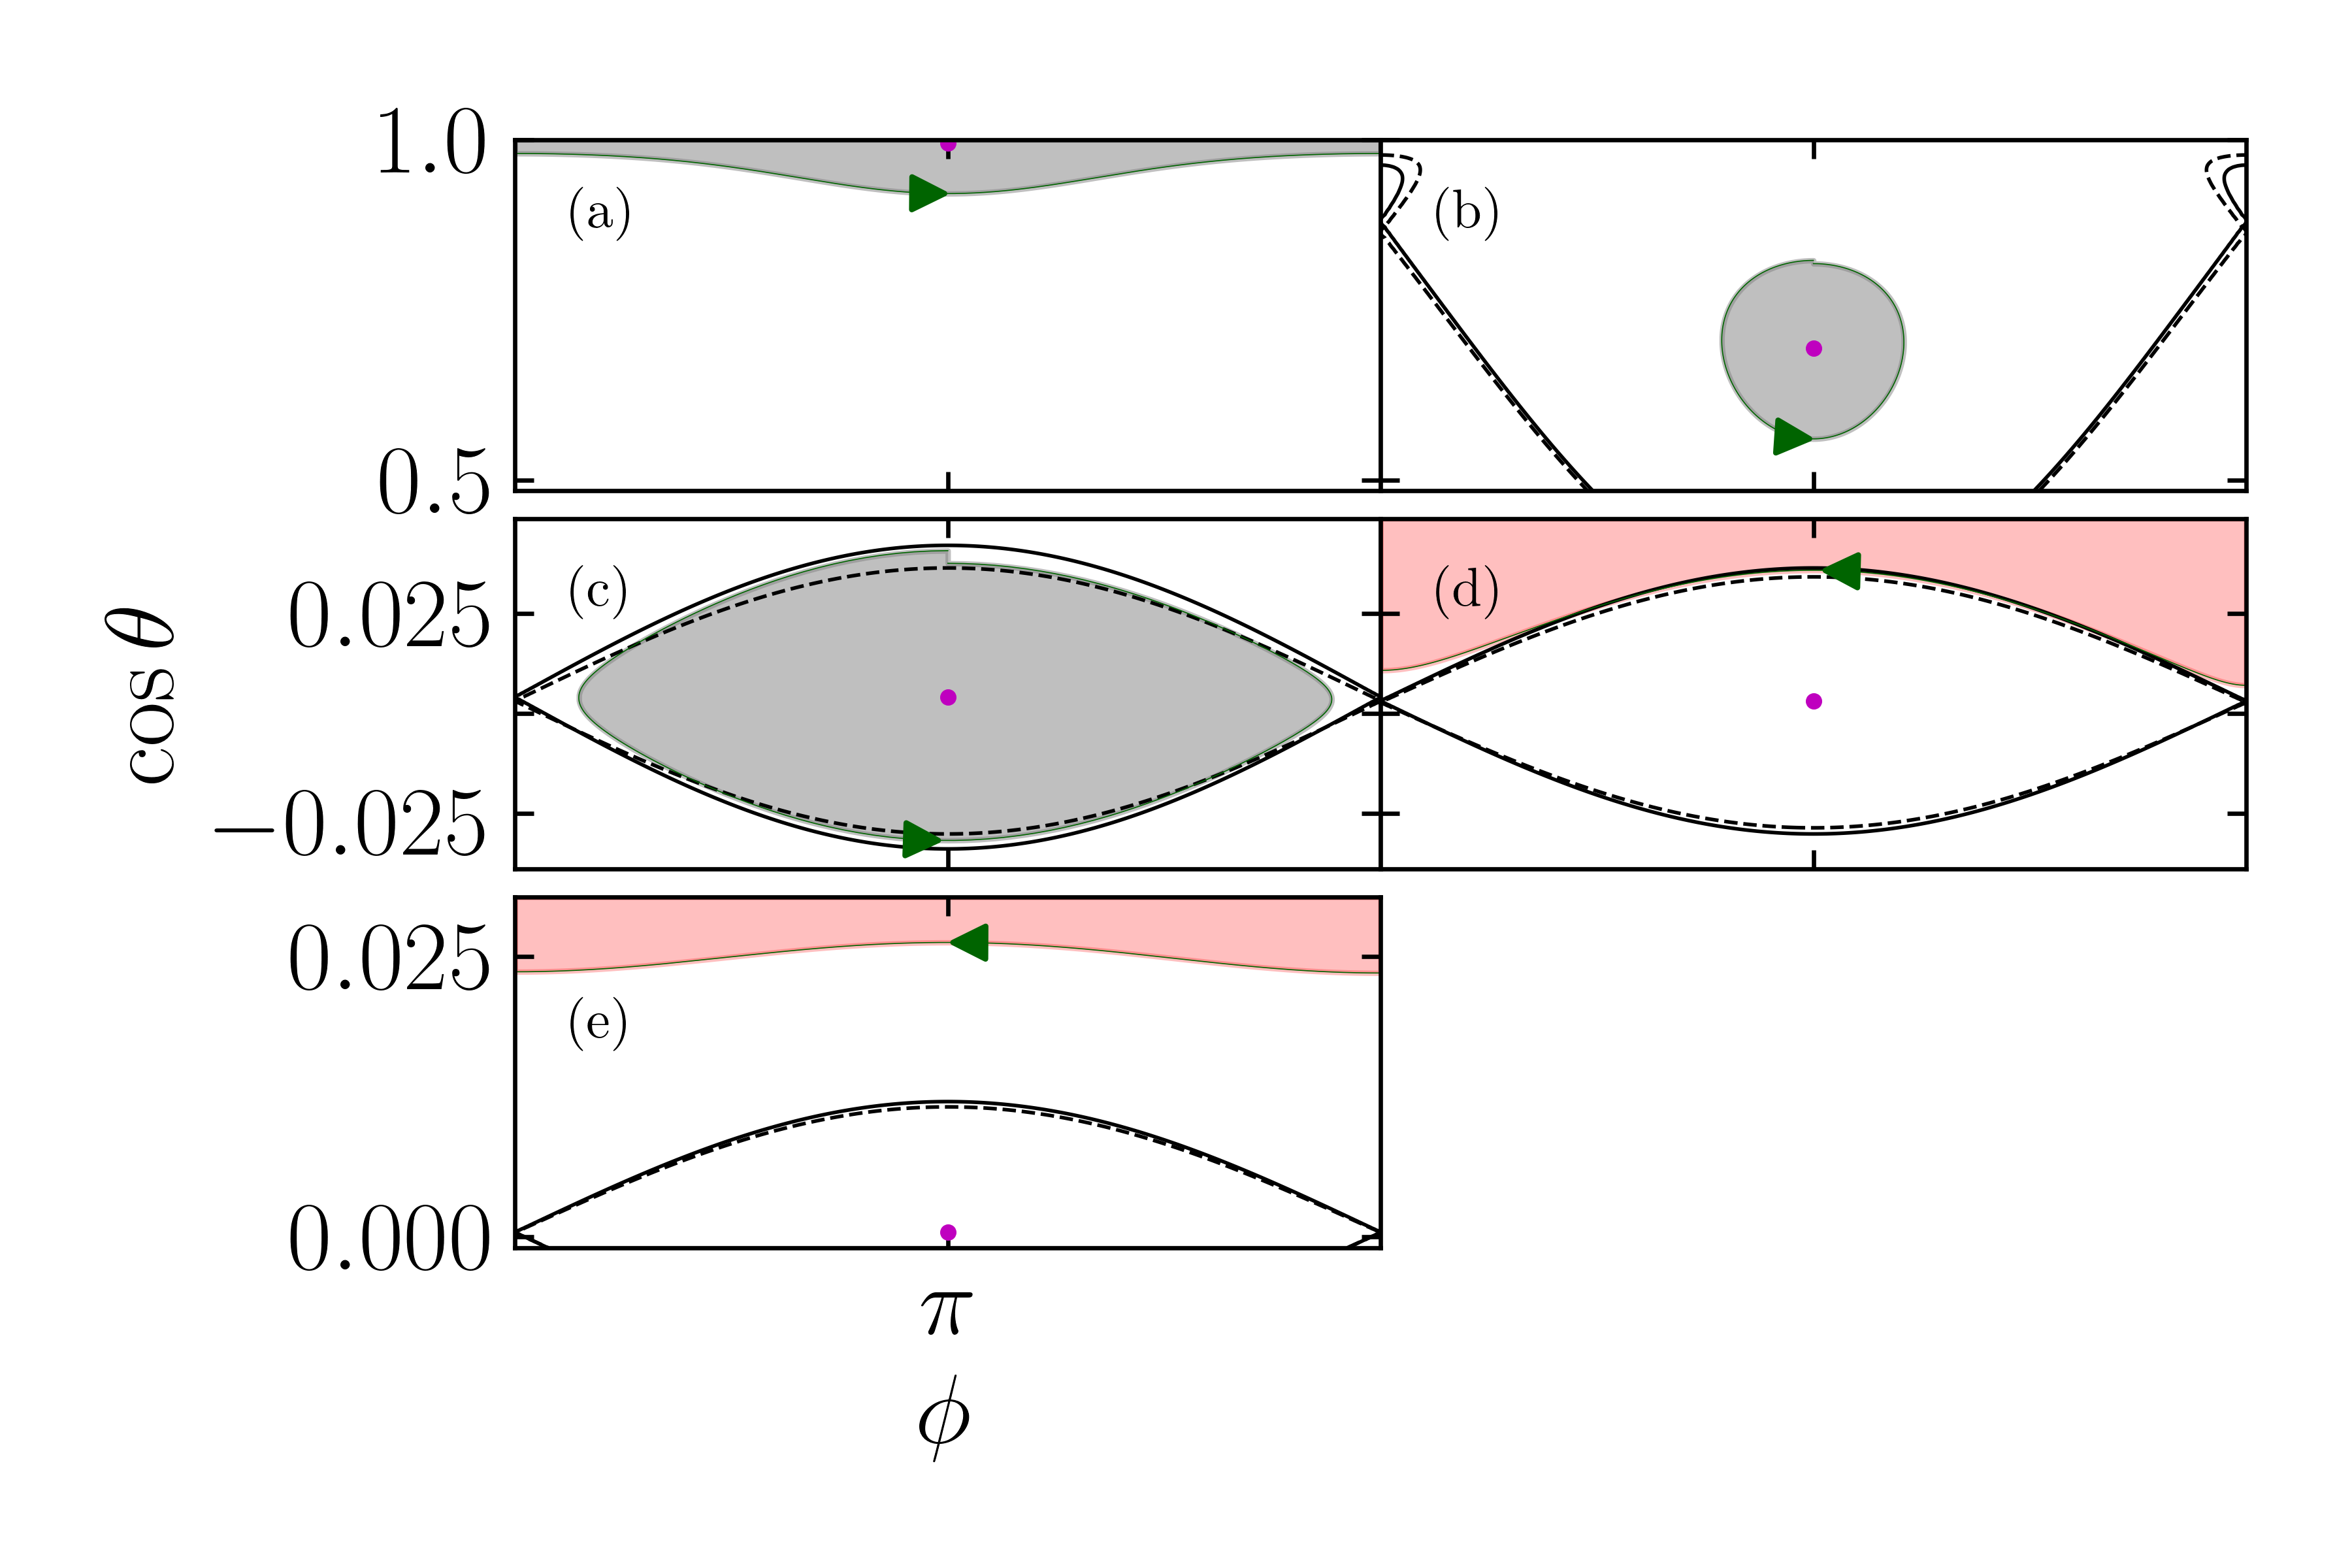
\includegraphics[width=\textwidth]{../../initial/2_toy2/3testo21_subplots.png}
            \end{figure}
        \end{column}
    \end{columns}
    Thus, $\theta_{sd, i} \equiv \hat{s}(t = 0) \cdot \hat{l}_d \approx 0
    \Rightarrow \theta_f \approx 90^\circ$.
\end{frame}

\begin{frame}
    \frametitle{Adiabatic Dynamics}
    \framesubtitle{Zone Transition Histories}

    \begin{columns}
        \begin{column}{0.5\textwidth}
            \begin{figure}
                \centering
                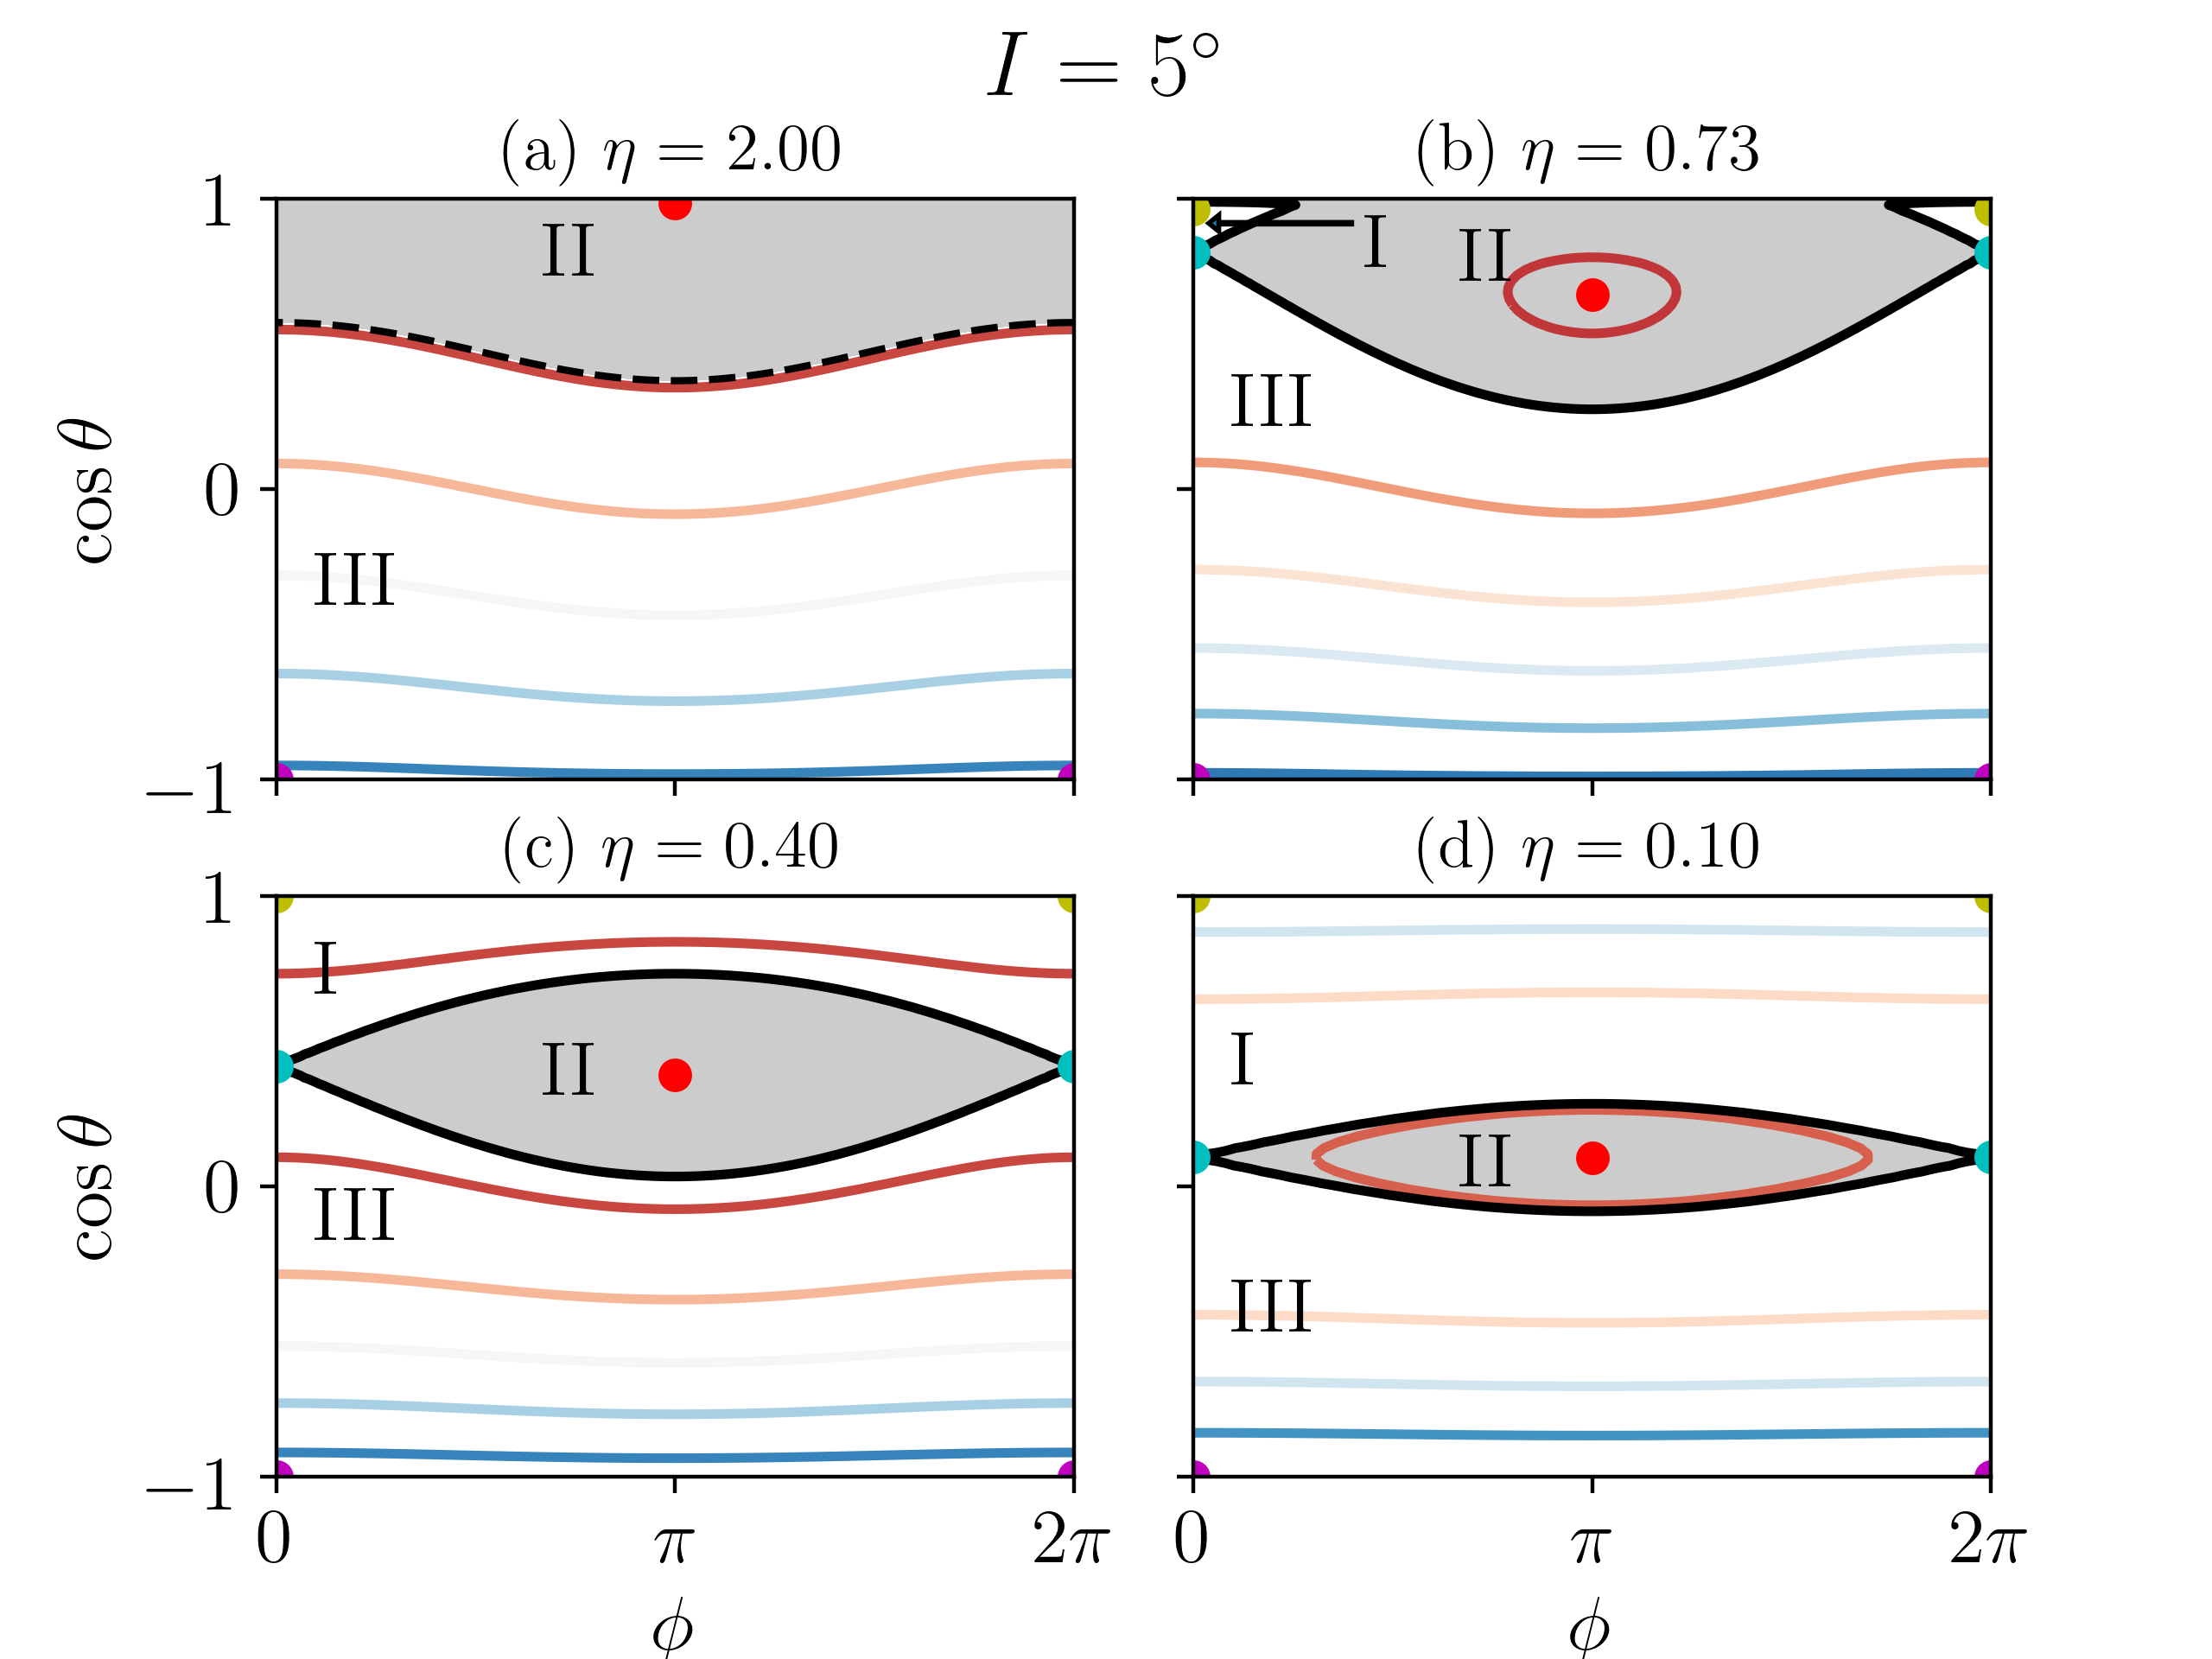
\includegraphics[width=\textwidth]{../../initial/0_eta/1contours_flip.png}
            \end{figure}
        \end{column}
        \begin{column}{0.5\textwidth}
            \begin{itemize}
                \item Start in $\z*{II, III}$, end in $\z*{I, III}$.
                    \emph{Must cross zones.}

                \item Expected transitions:
                    \begin{itemize}
                        \item $\mathbf{II \to I}$
                        \item $II \to III$
                        \item $III \to I$
                        \item $III \to III$
                        \item $\p*{III \to II \to I}$
                    \end{itemize}
            \end{itemize}
        \end{column}
    \end{columns}
\end{frame}

\begin{frame}
    \frametitle{Adiabatic Dynamics}
    \framesubtitle{Adiabatic Resonance Advection $II \to III$}

    \begin{columns}
        \begin{column}{0.5\textwidth}
            \begin{figure}[t]
                \centering
                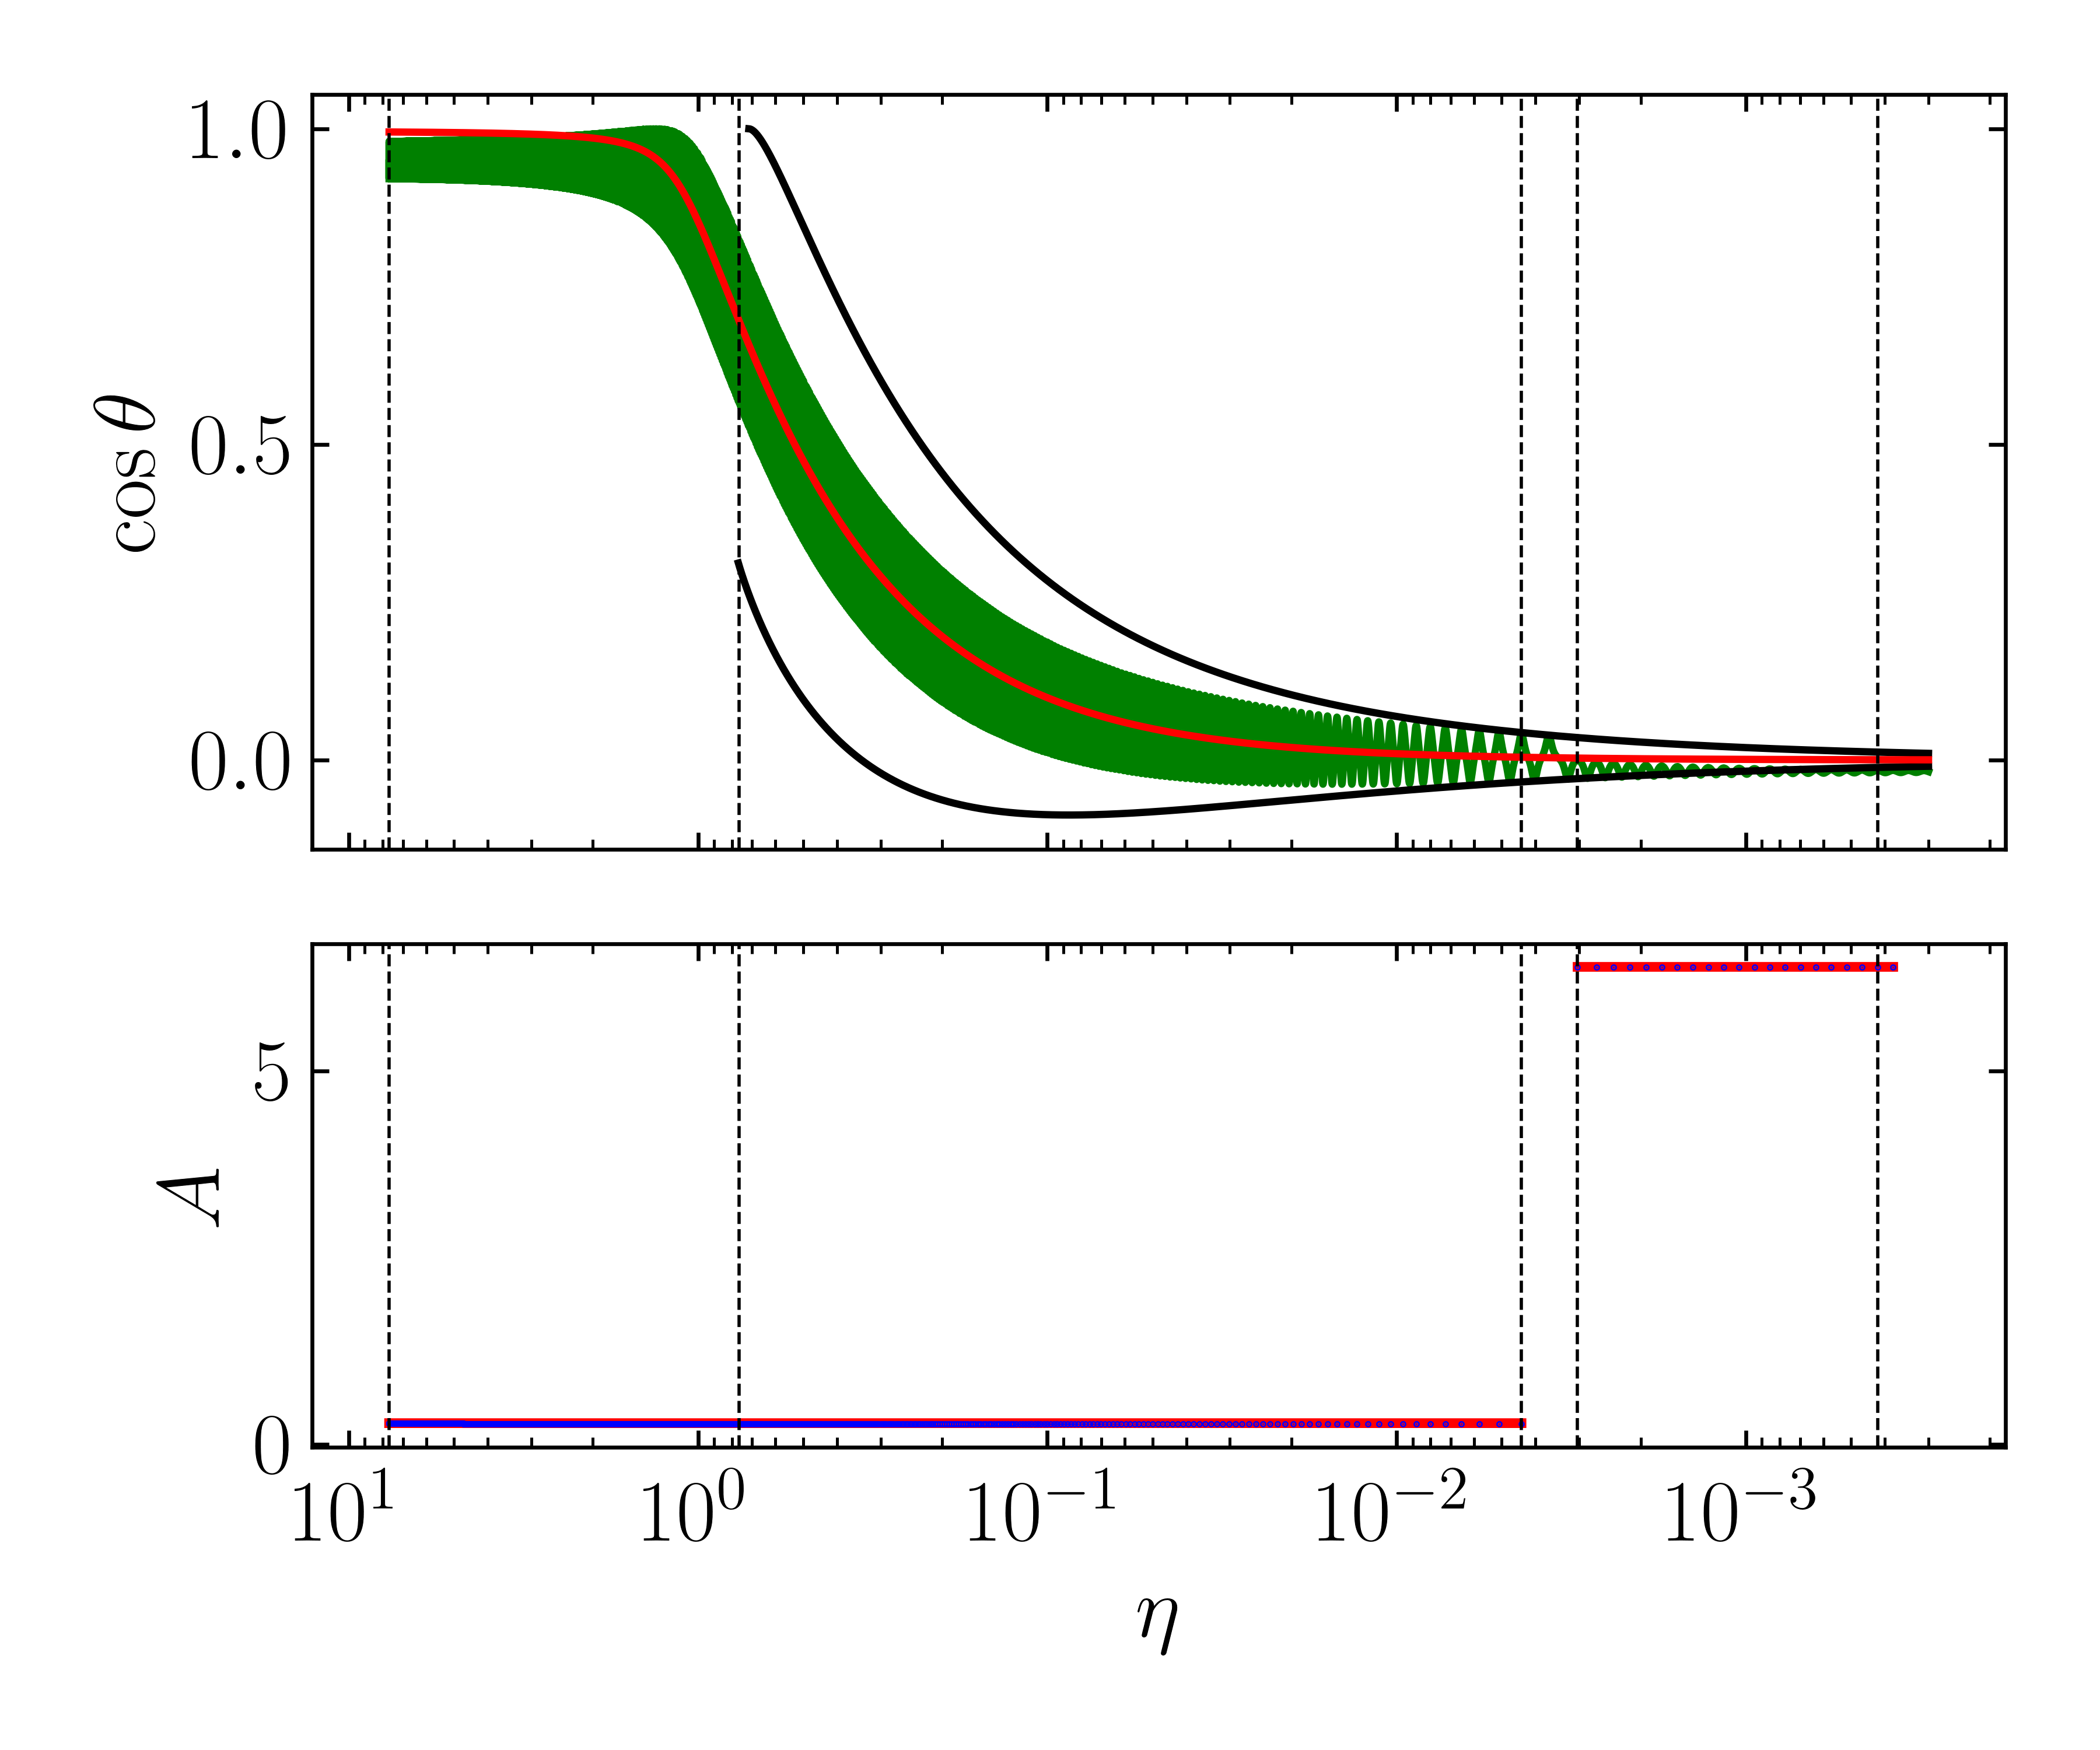
\includegraphics[width=\textwidth]{../../initial/2_toy2/3testo23.png}
            \end{figure}
        \end{column}
        \begin{column}{0.5\textwidth}
            \begin{figure}[t]
                \centering
                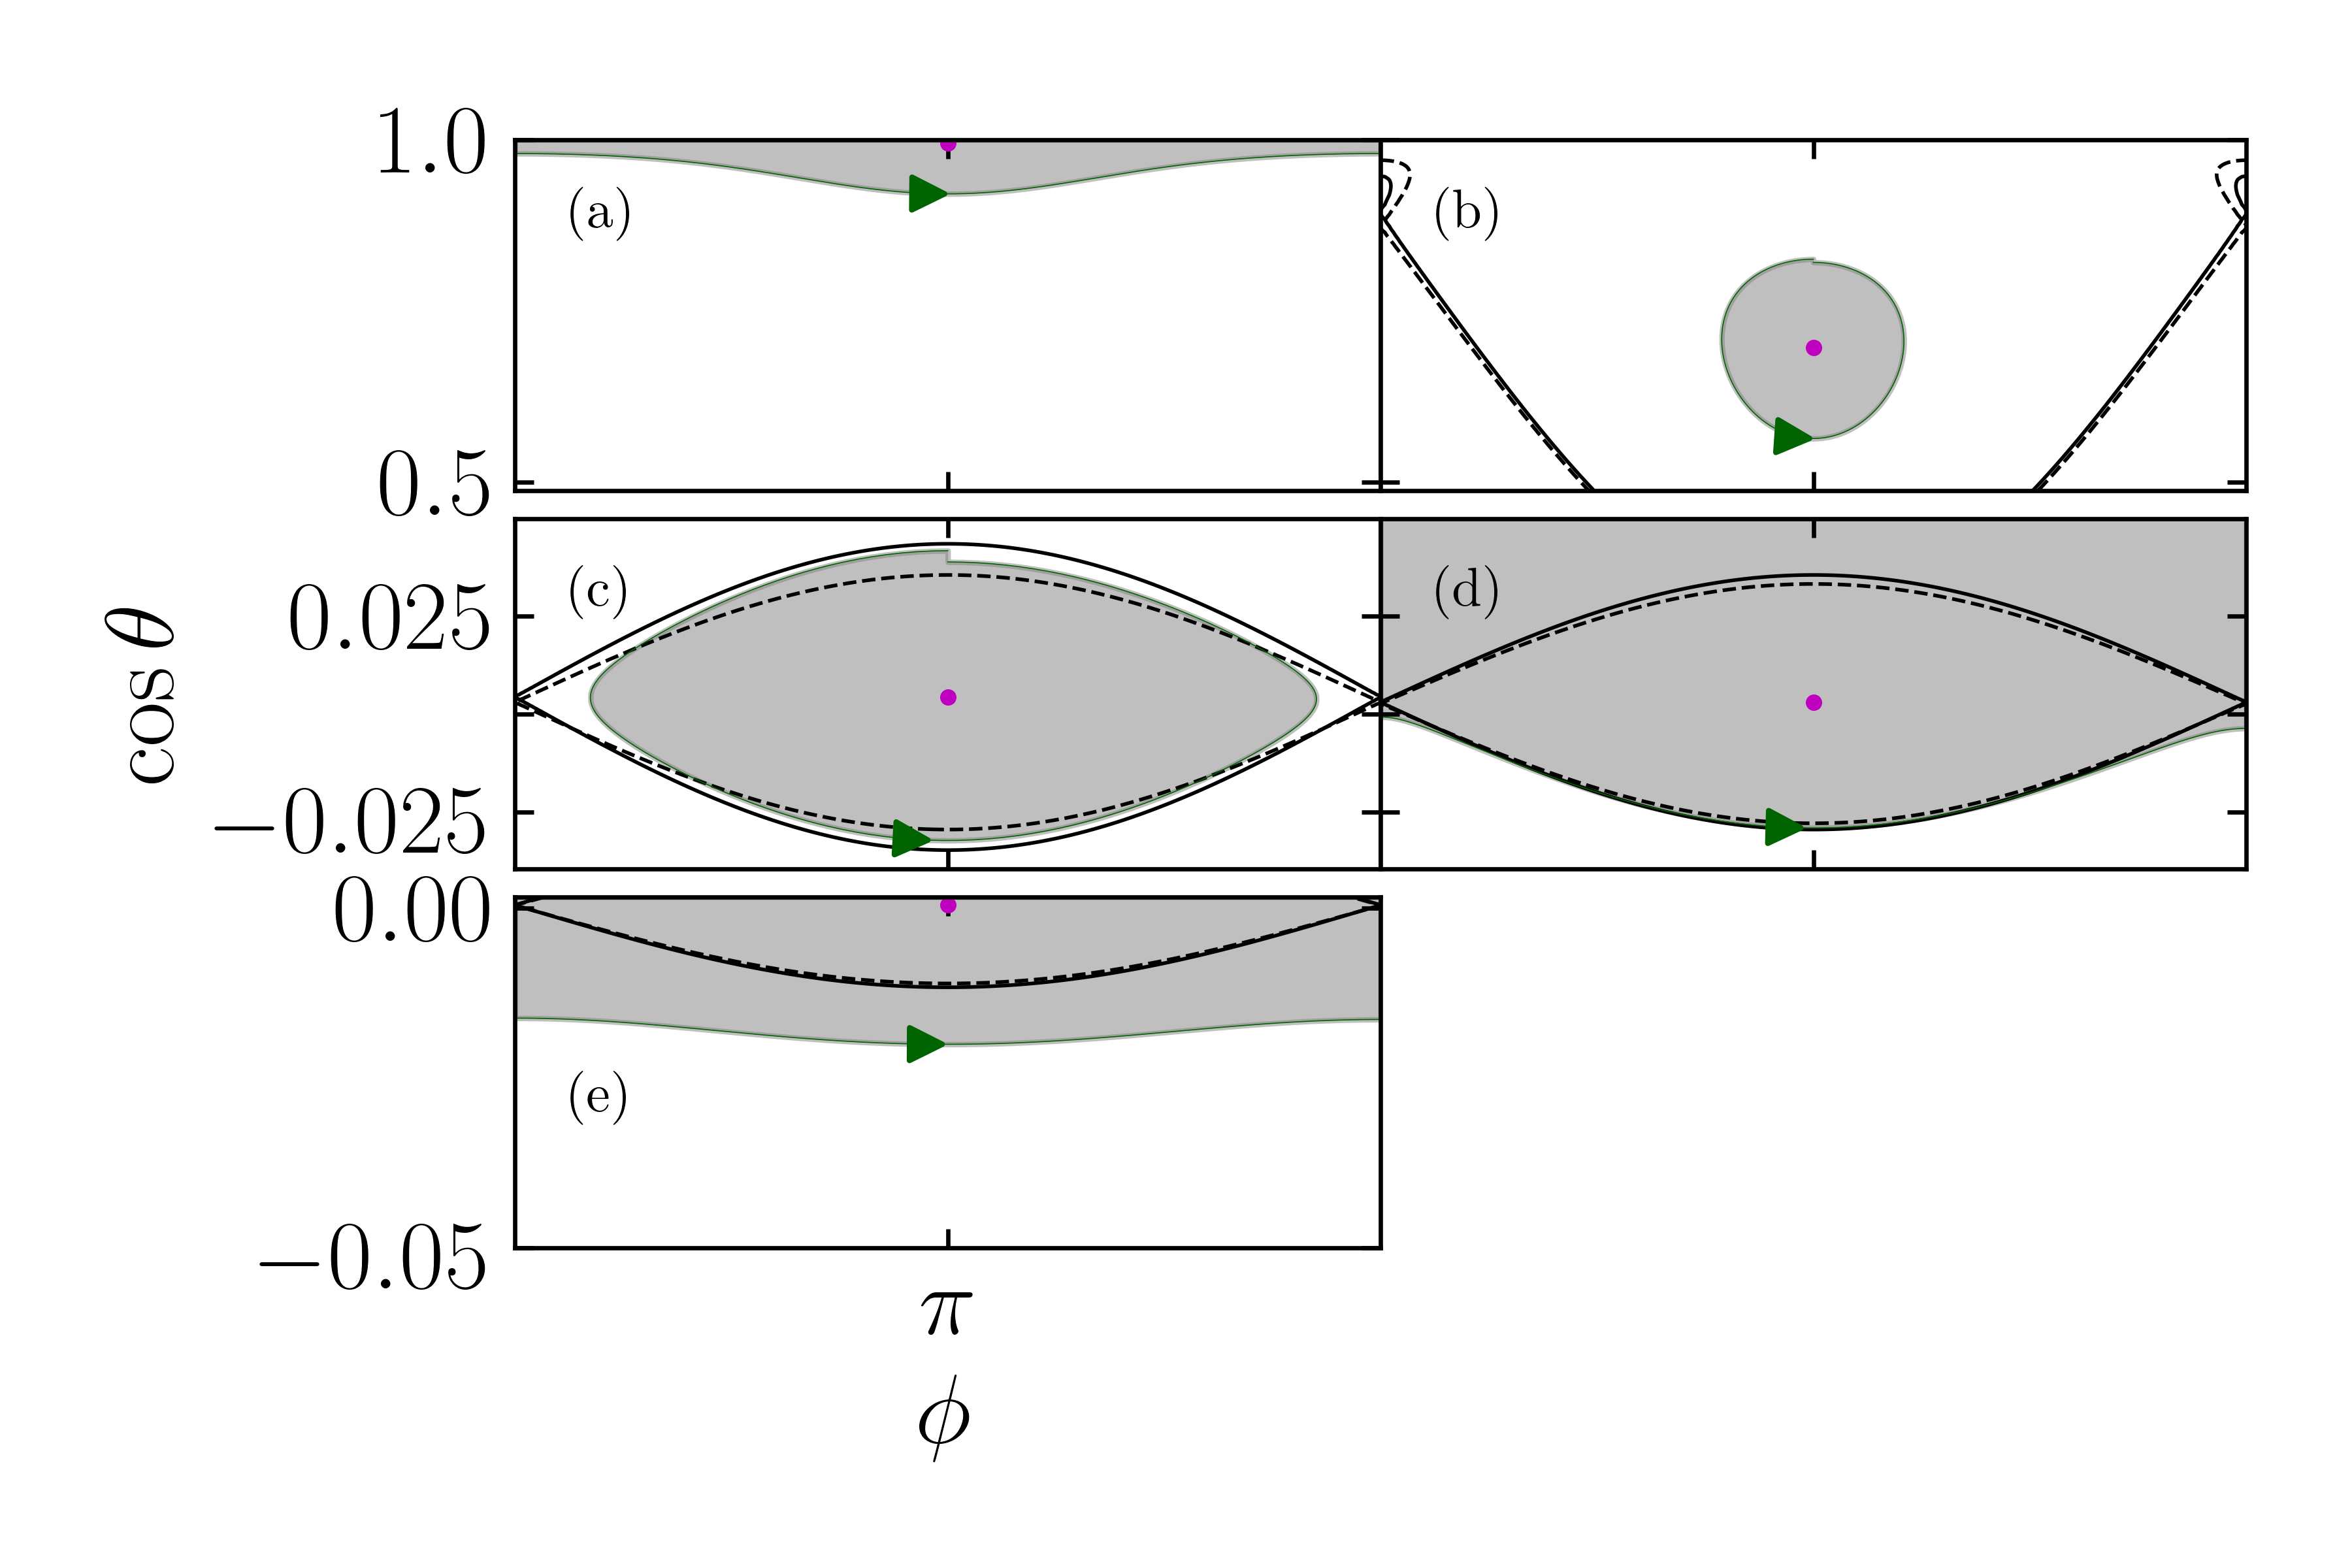
\includegraphics[width=\textwidth]{../../initial/2_toy2/3testo23_subplots.png}
            \end{figure}
        \end{column}
    \end{columns}
\end{frame}

\begin{frame}
    \frametitle{Adiabatic Dynamics}
    \framesubtitle{Adiabatic Resonance Advection $III \to I$}

    \begin{columns}
        \begin{column}{0.5\textwidth}
            \begin{figure}[t]
                \centering
                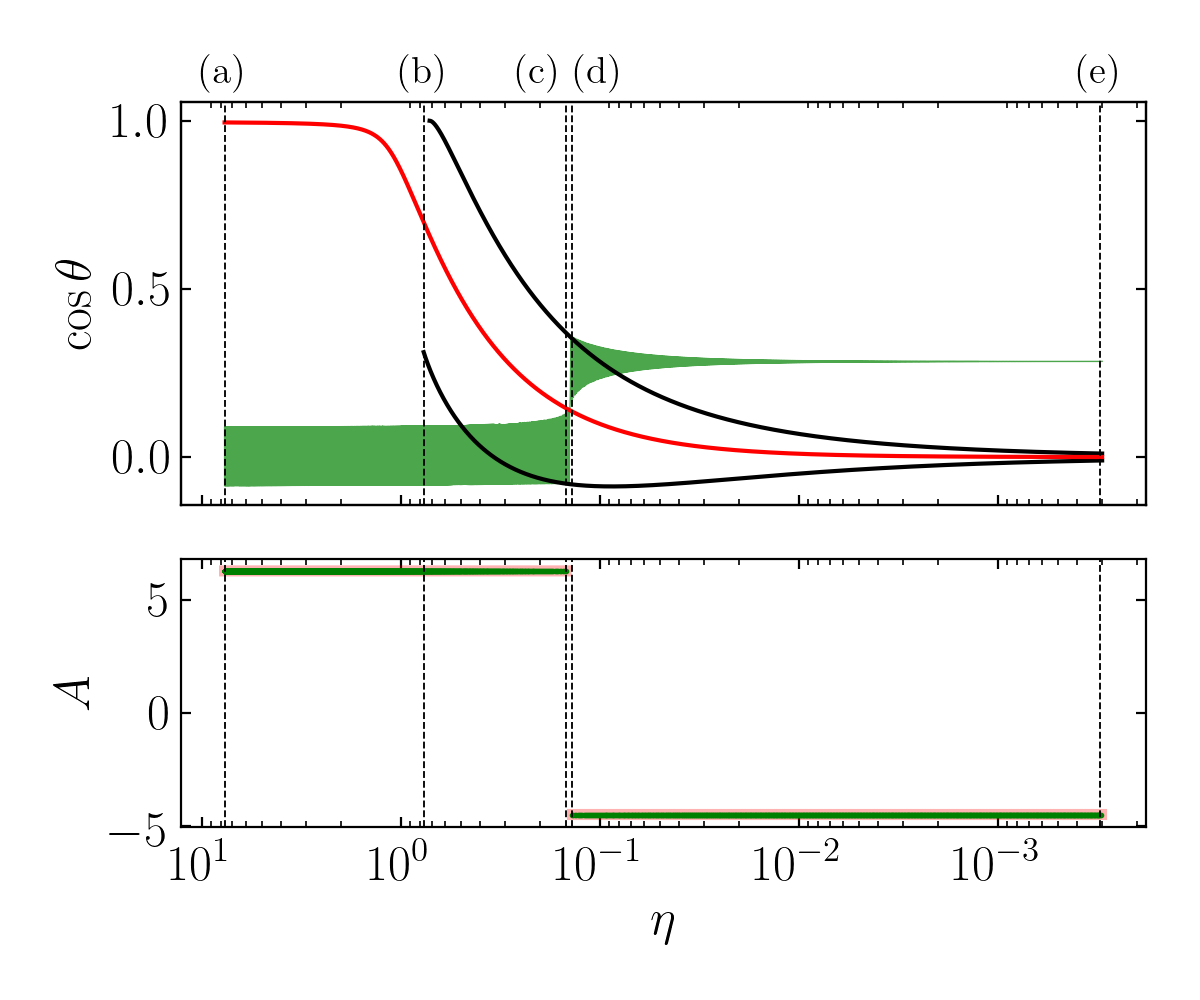
\includegraphics[width=\textwidth]{../../initial/2_toy2/3testo31.png}
            \end{figure}
        \end{column}
        \begin{column}{0.5\textwidth}
            \begin{figure}[t]
                \centering
                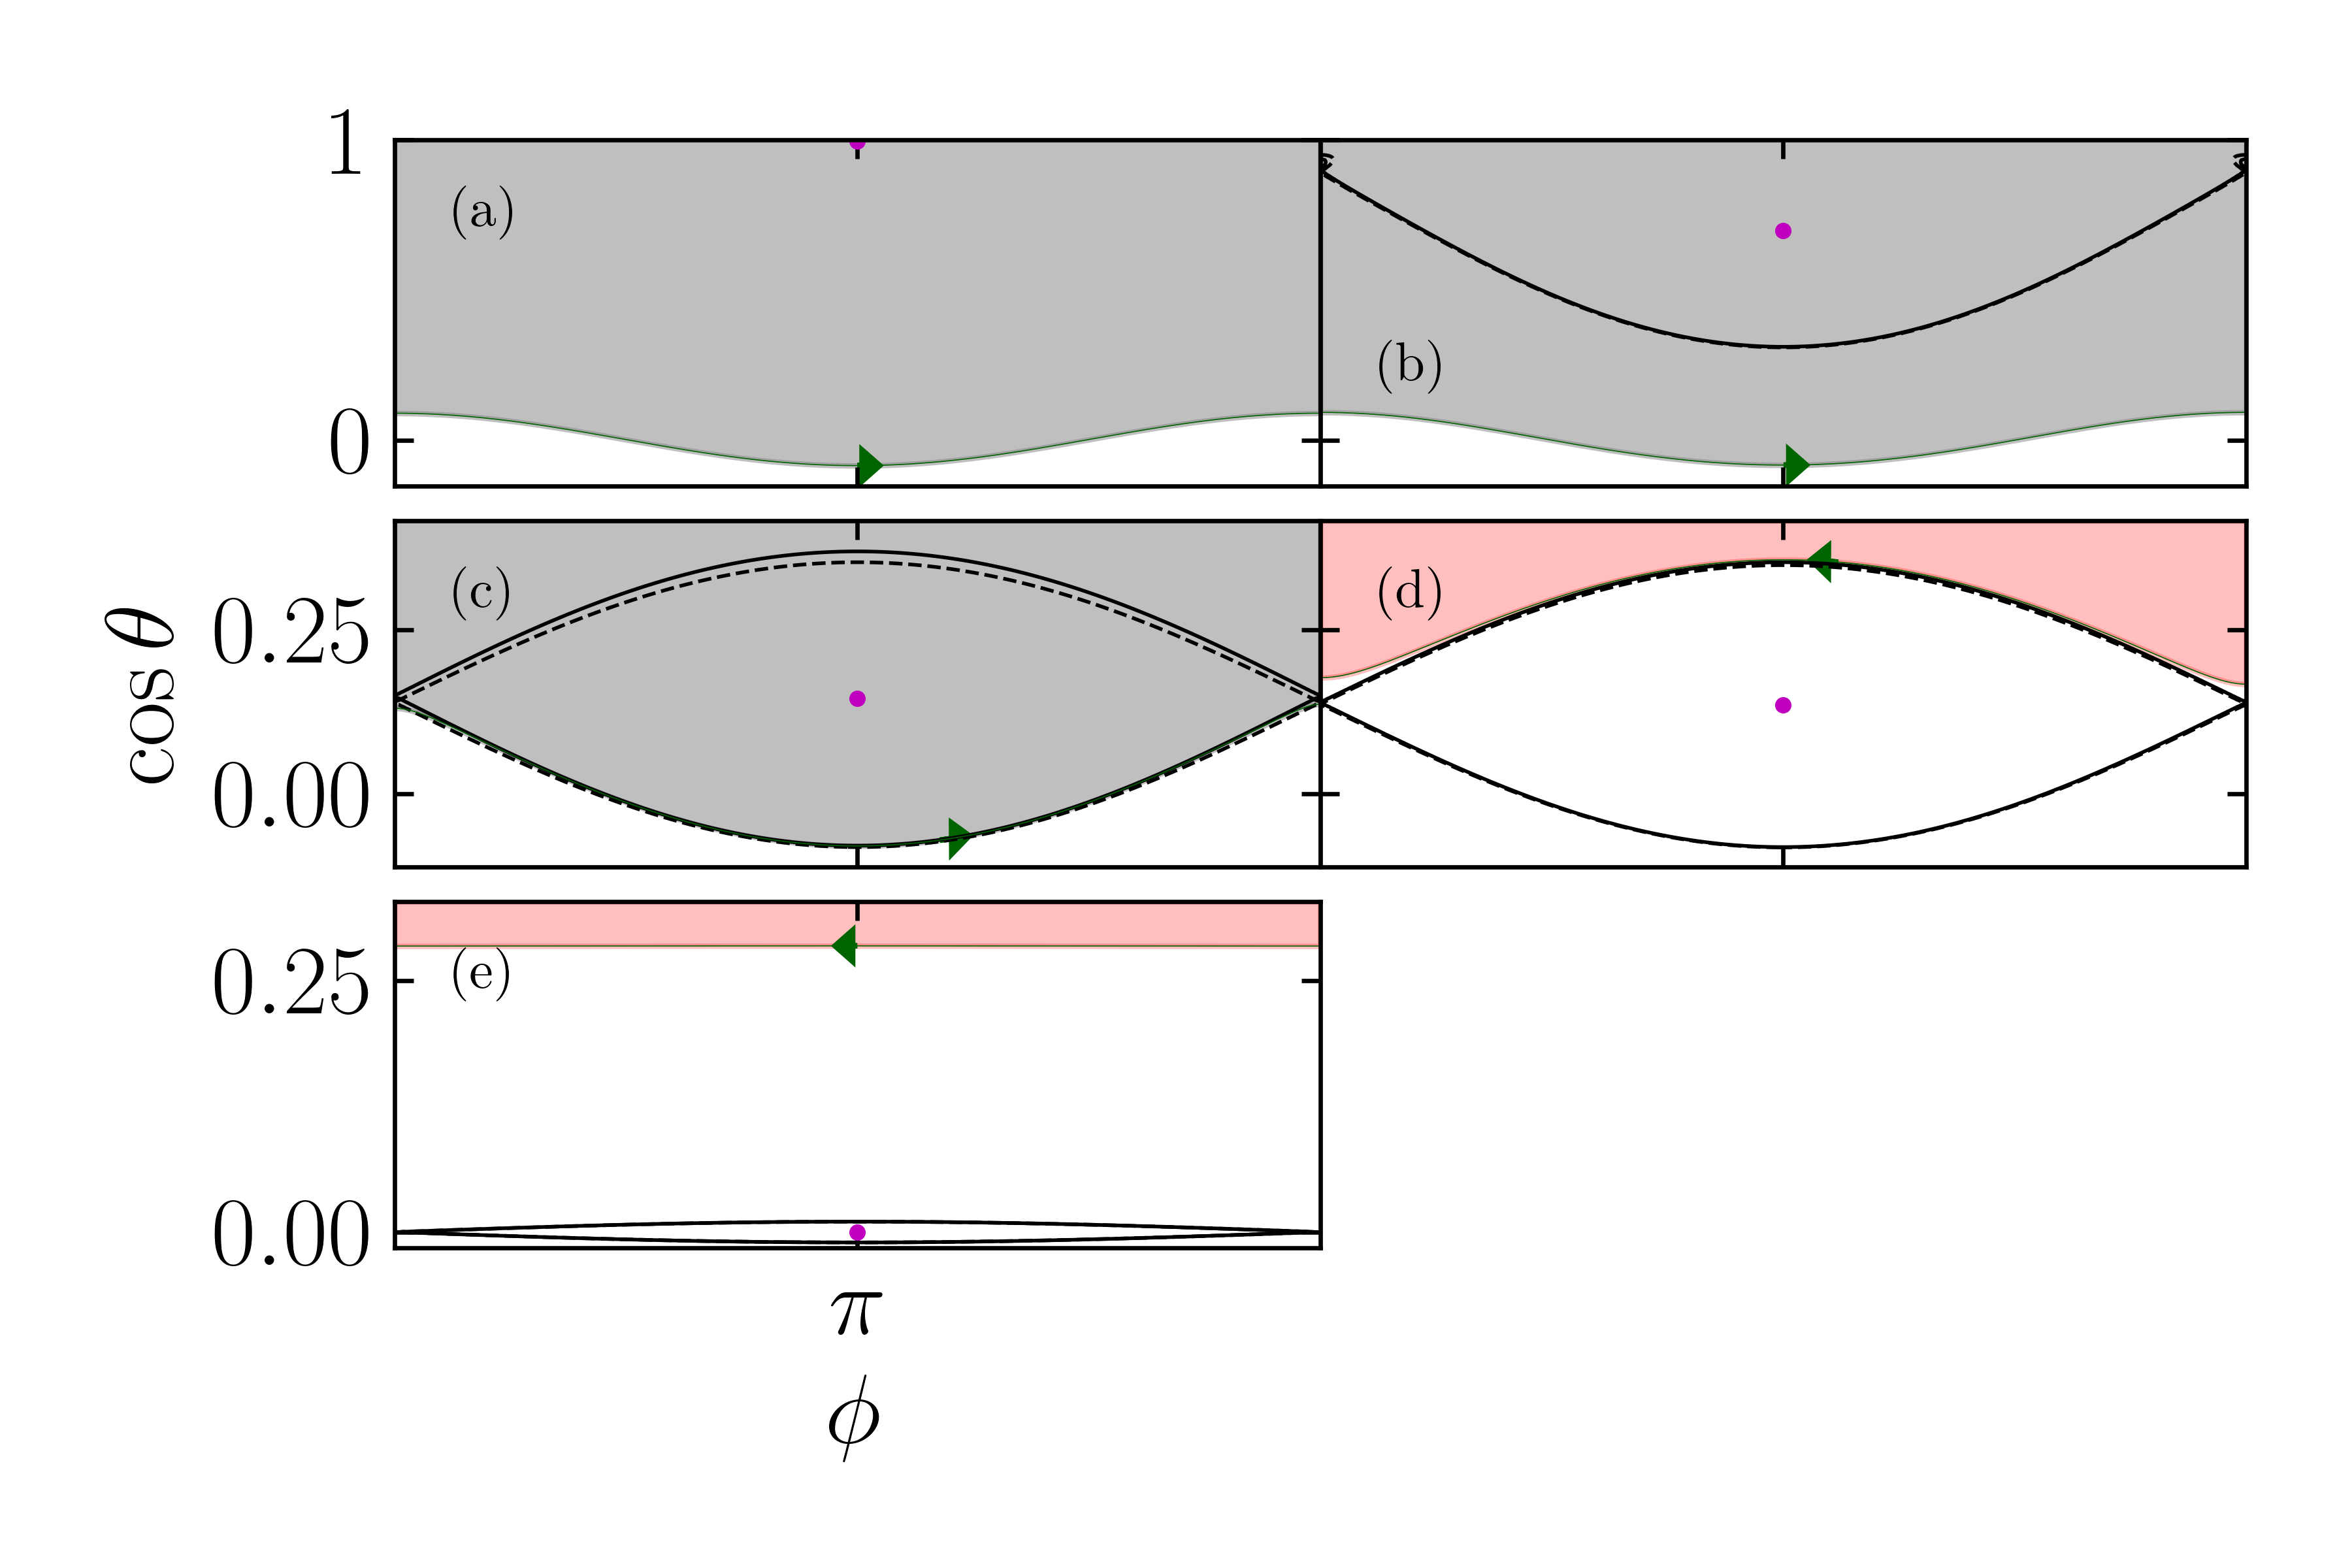
\includegraphics[width=\textwidth]{../../initial/2_toy2/3testo31_subplots.png}
            \end{figure}
        \end{column}
    \end{columns}
\end{frame}

\begin{frame}
    \frametitle{Adiabatic Dynamics}
    \framesubtitle{Adiabatic Resonance Advection $III \to II \to I$}

    \begin{columns}
        \begin{column}{0.5\textwidth}
            \begin{figure}[t]
                \centering
                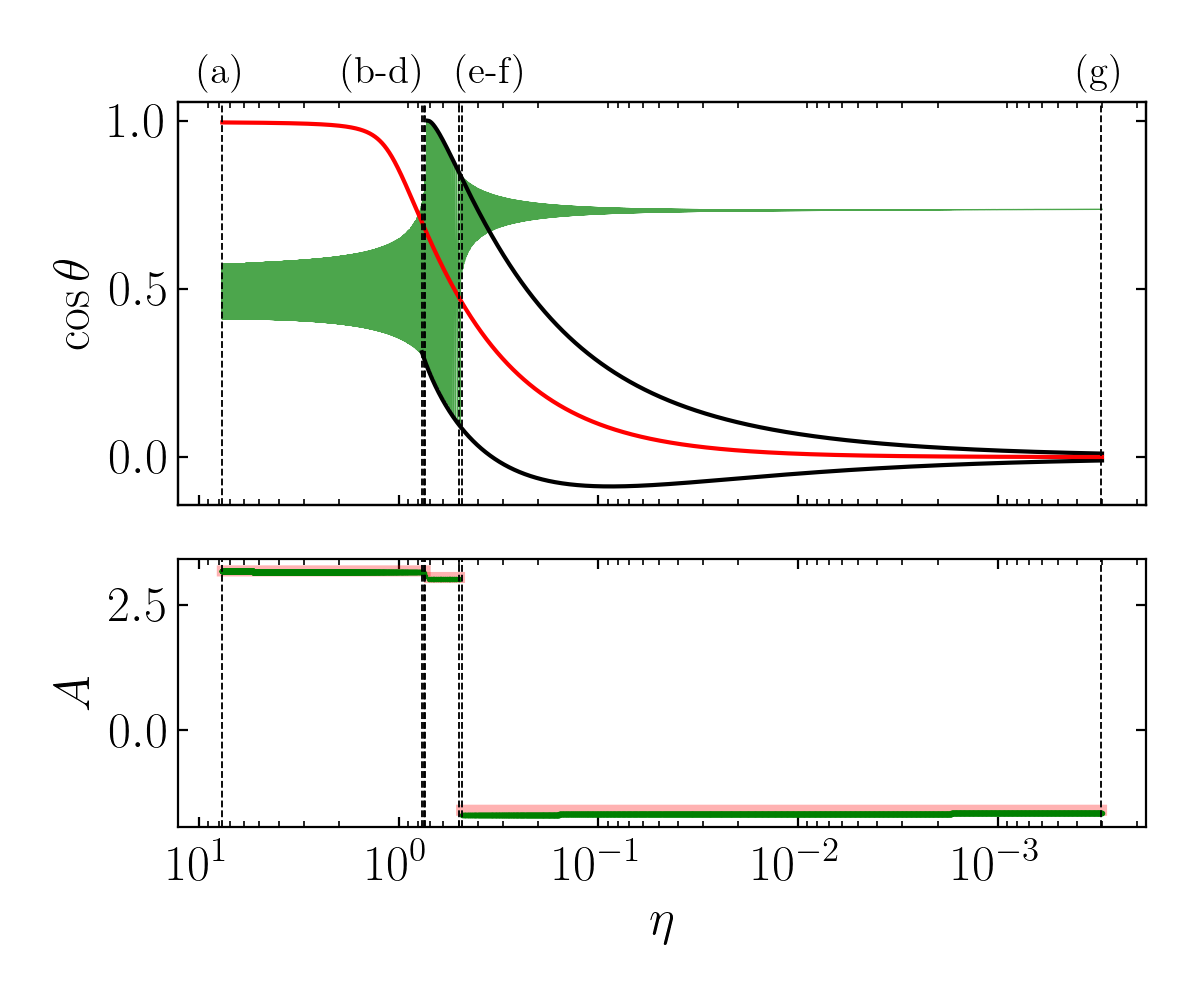
\includegraphics[width=\textwidth]{../../initial/2_toy2/3testo321.png}
            \end{figure}
        \end{column}
        \begin{column}{0.5\textwidth}
            \begin{figure}[t]
                \centering
                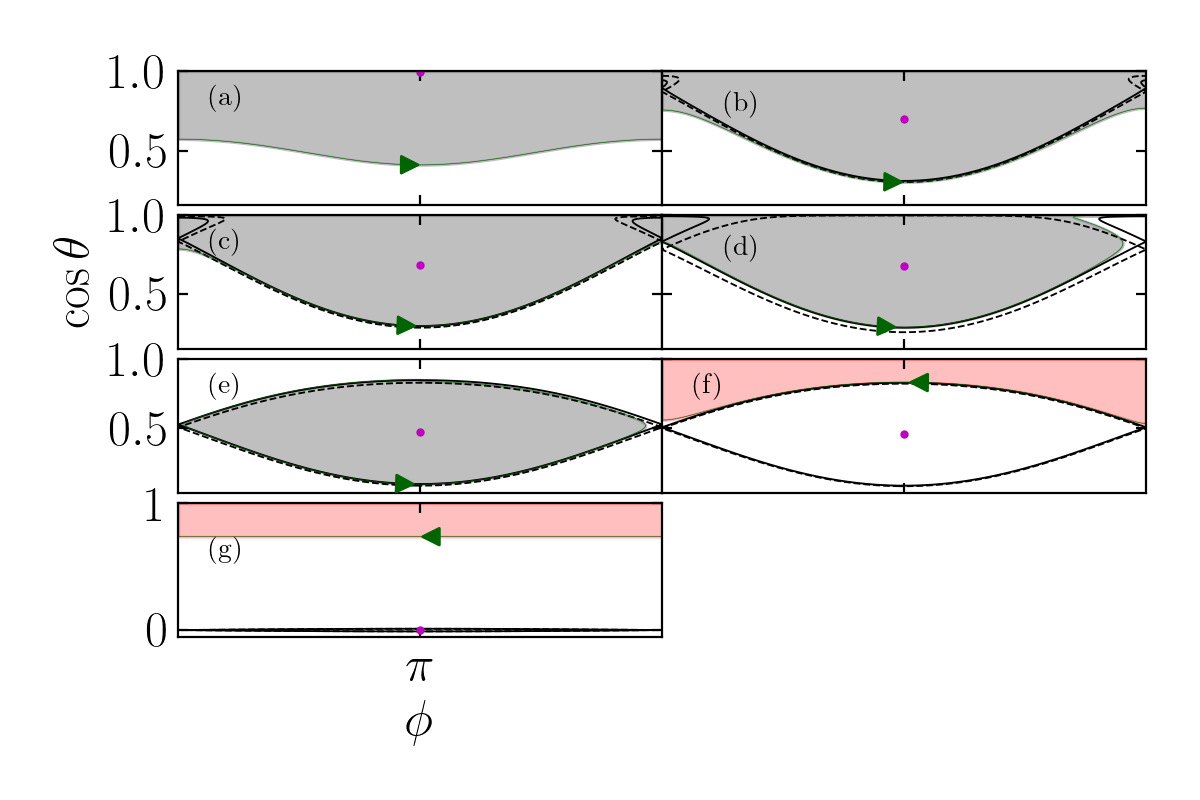
\includegraphics[width=\textwidth]{../../initial/2_toy2/3testo321_subplots.png}
            \end{figure}
        \end{column}
    \end{columns}
\end{frame}

\begin{frame}
    \frametitle{Adiabatic Dynamics}
    \framesubtitle{Distribution}
    {\small
    \begin{itemize}
        \item Zone crossing is \emph{probabilistic}, solved (Henrard 1982).
        \item $\cos \theta_f \approx \p*{\frac{\pi \theta_{sd,i}^2}{16}}^2 \cot
            I \pm \frac{\theta_{sd,i}^2}{4}$
    \end{itemize}
    }
    \begin{figure}[t]
        \centering
        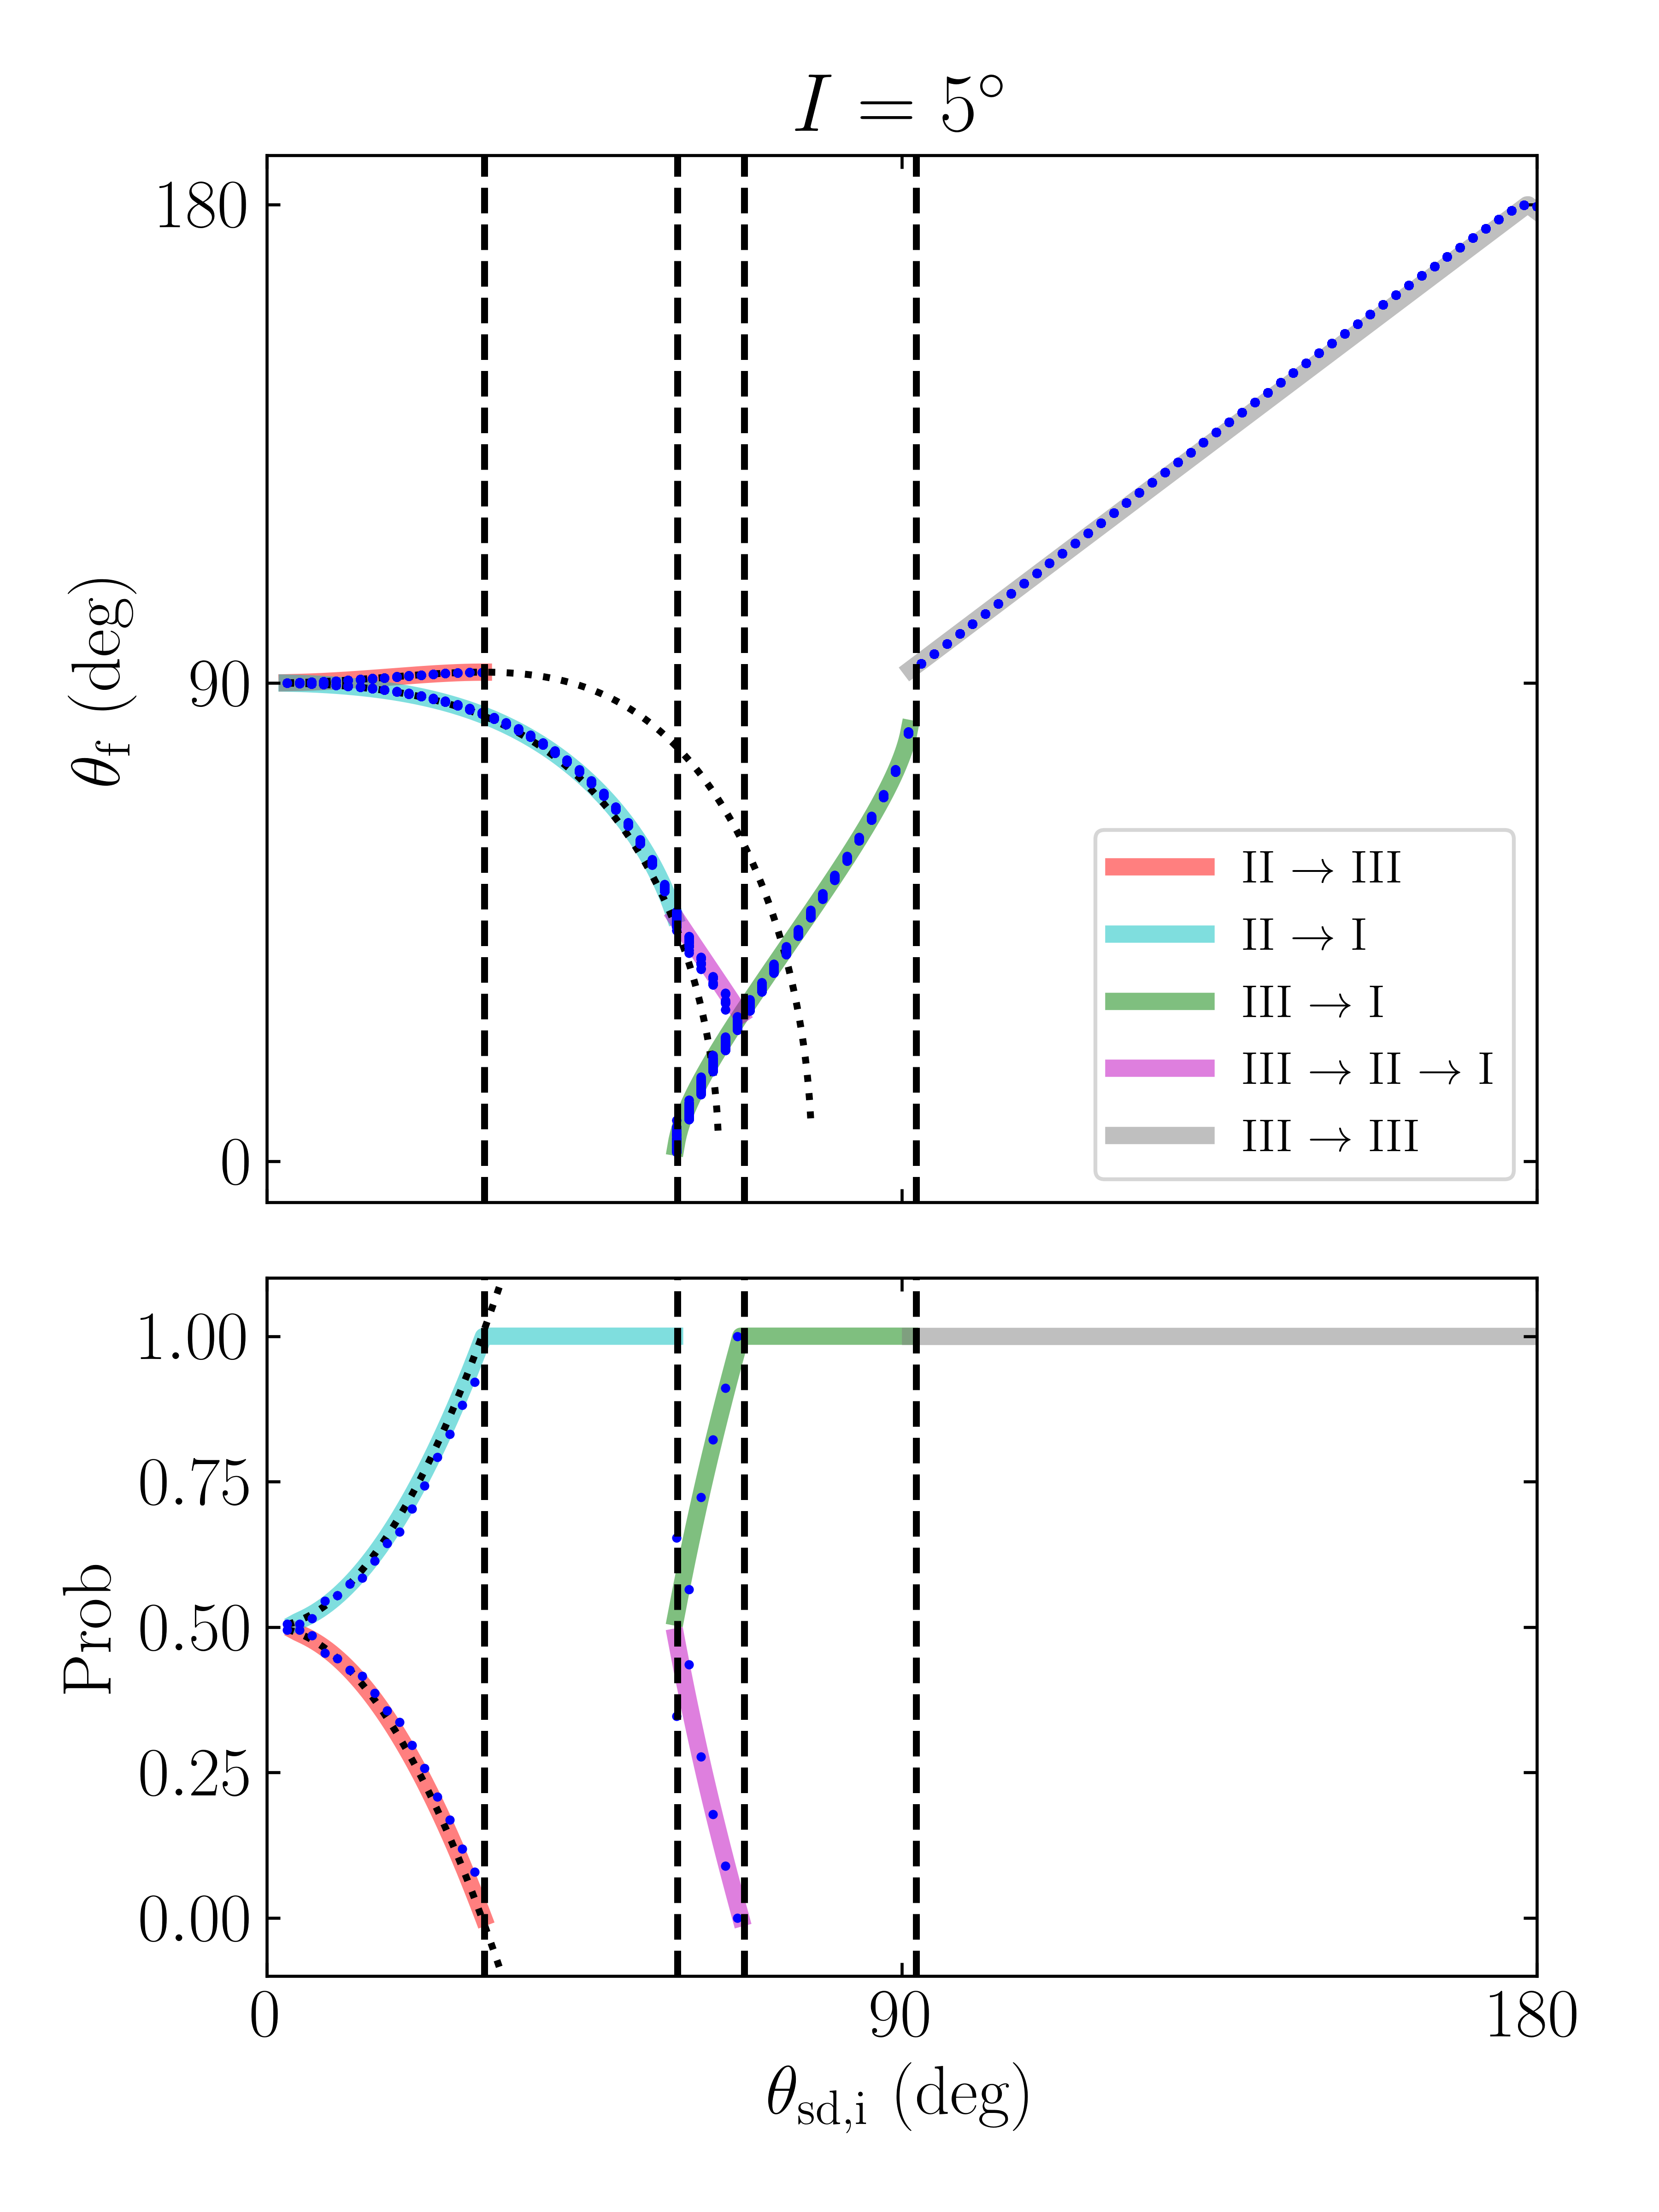
\includegraphics[width=0.65\textwidth]{../../initial/2_toy2/3_ensemble_05_35.png}
    \end{figure}
\end{frame}

\section{Effect of Non-adiabaticity}

\begin{frame}
    \frametitle{Effect of Non-adiabaticity}
    \framesubtitle{Breakdown of Adiabaticity}
    \begin{figure}[t]
        \centering
        \begin{subfigure}{0.45\textwidth}
            \centering
            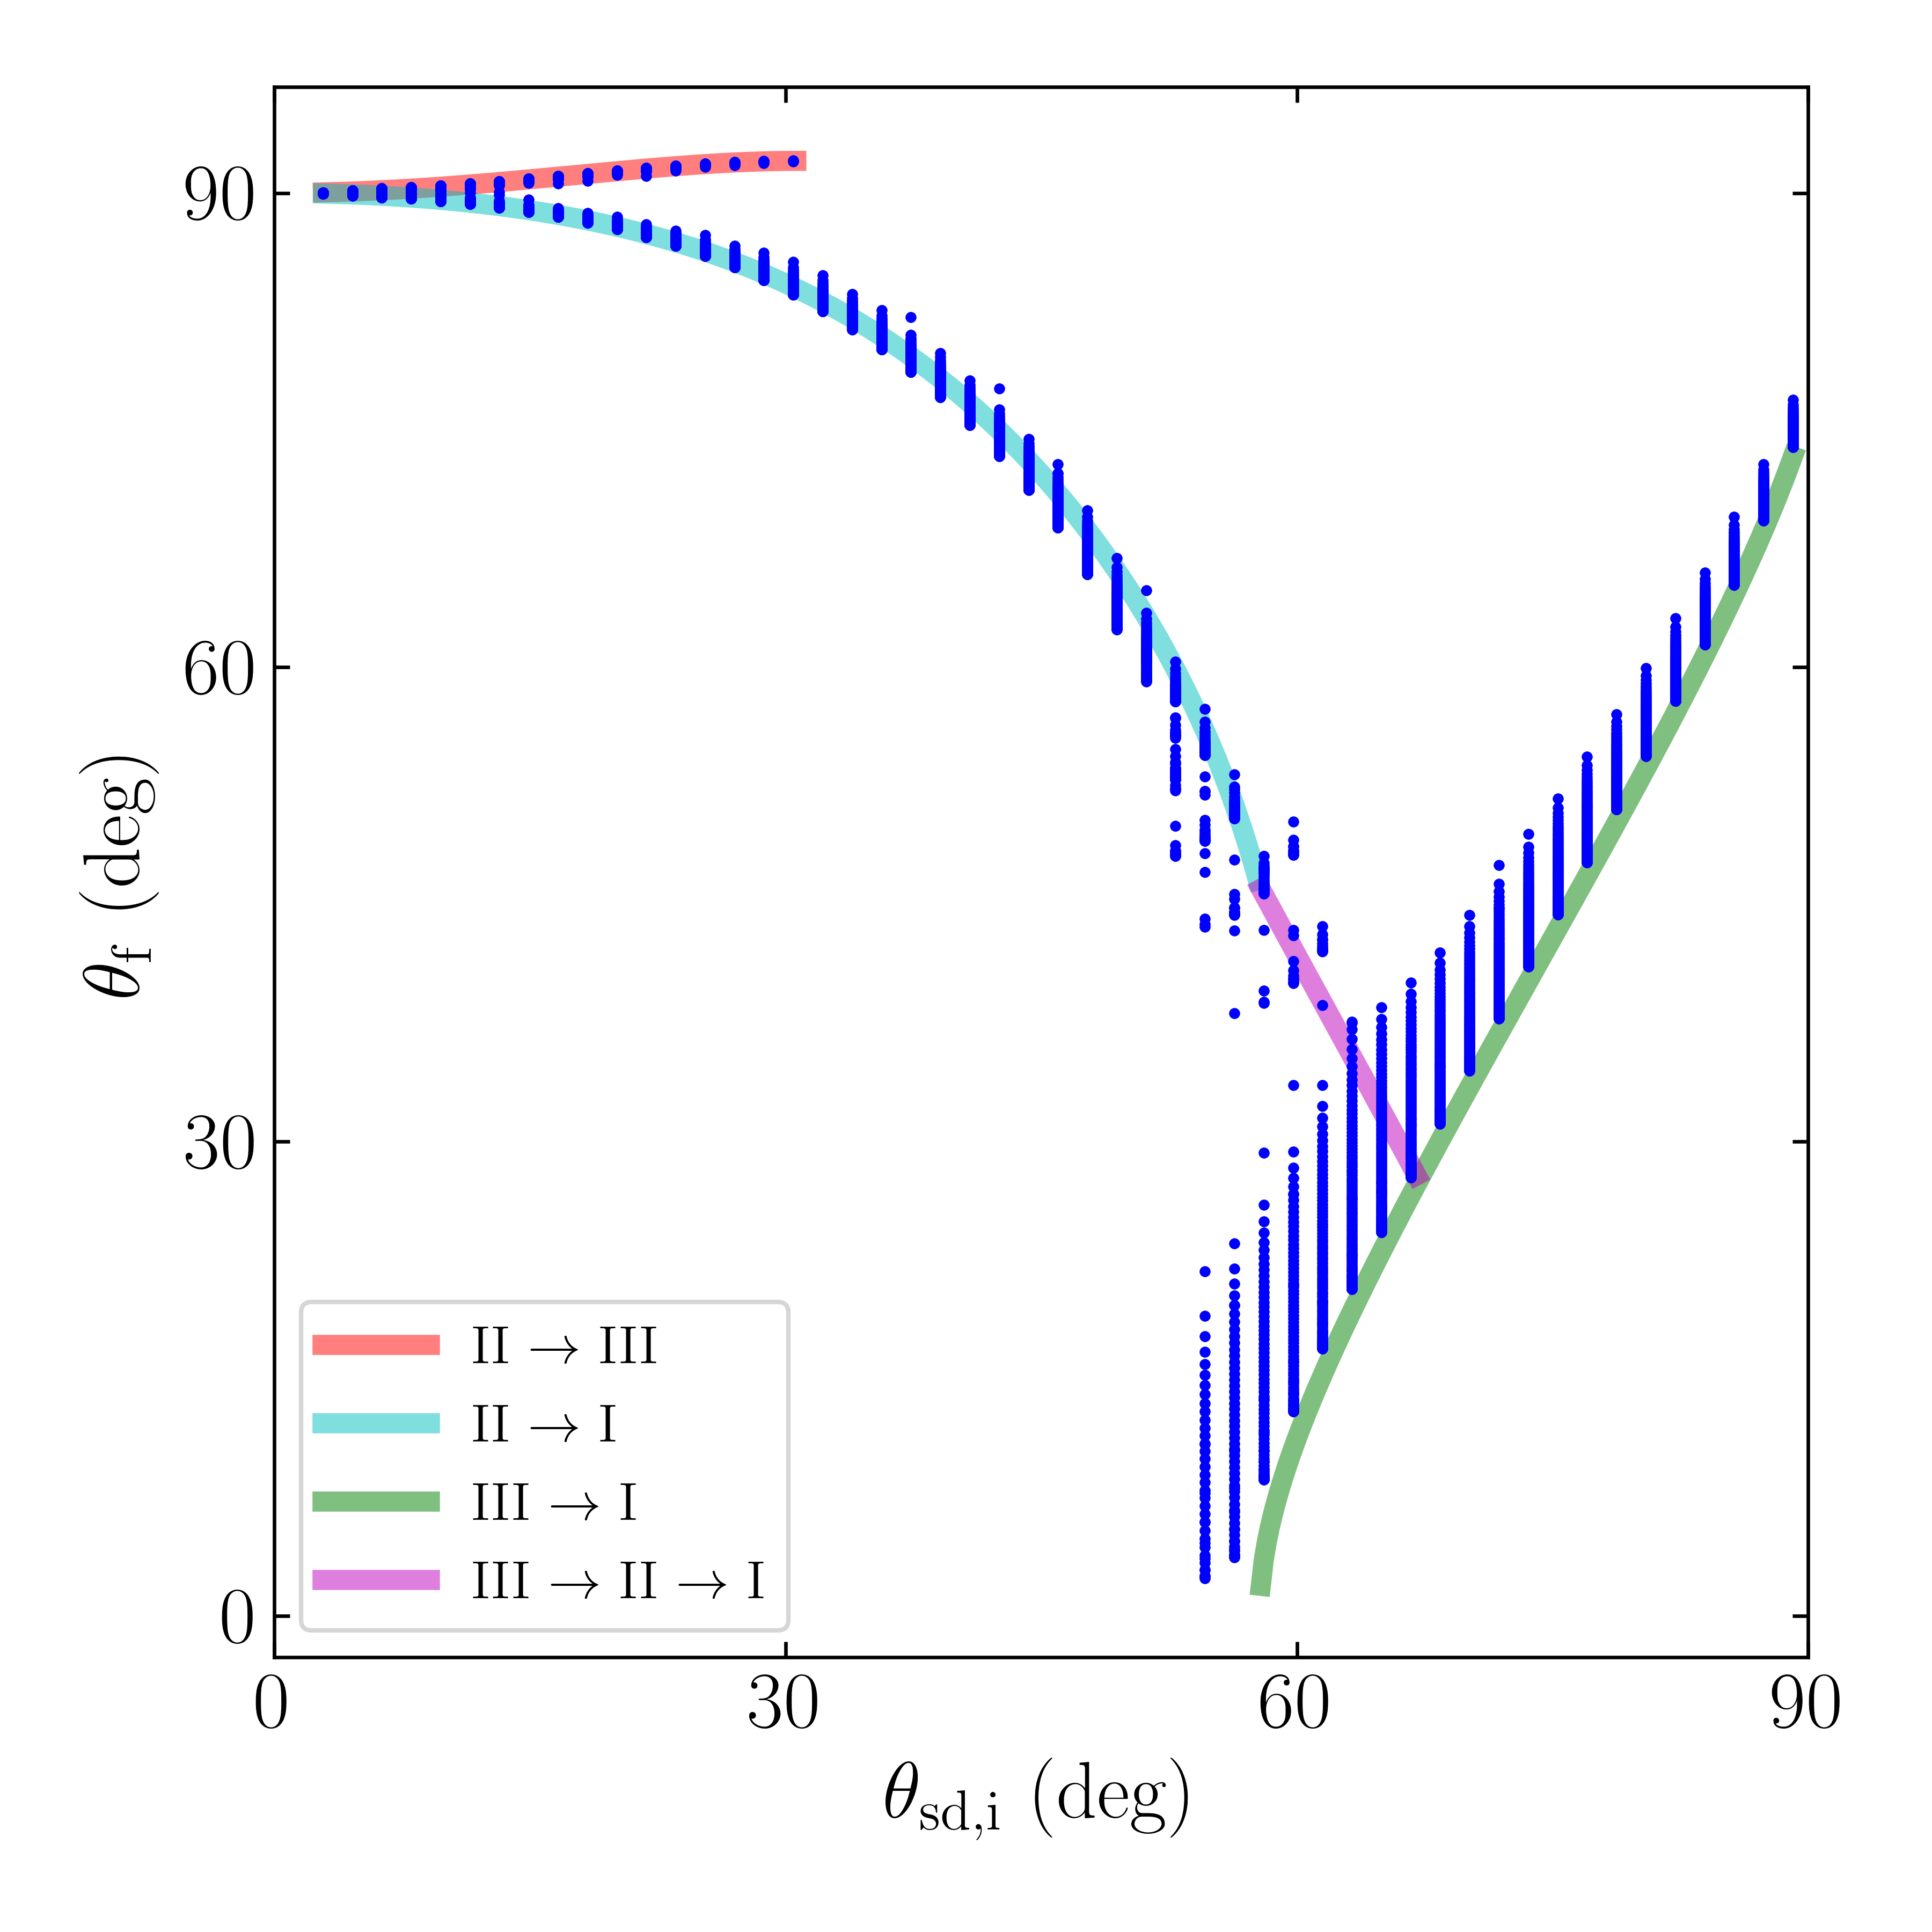
\includegraphics[width=0.8\textwidth]{../../initial/2_toy2/3_ensemble_05_25.png}
        \end{subfigure}
        \begin{subfigure}{0.45\textwidth}
            \centering
            \includegraphics[width=0.8\textwidth]{../../initial/2_toy2/3_ensemble_05_20.png}
        \end{subfigure}

        \begin{subfigure}{0.45\textwidth}
            \centering
            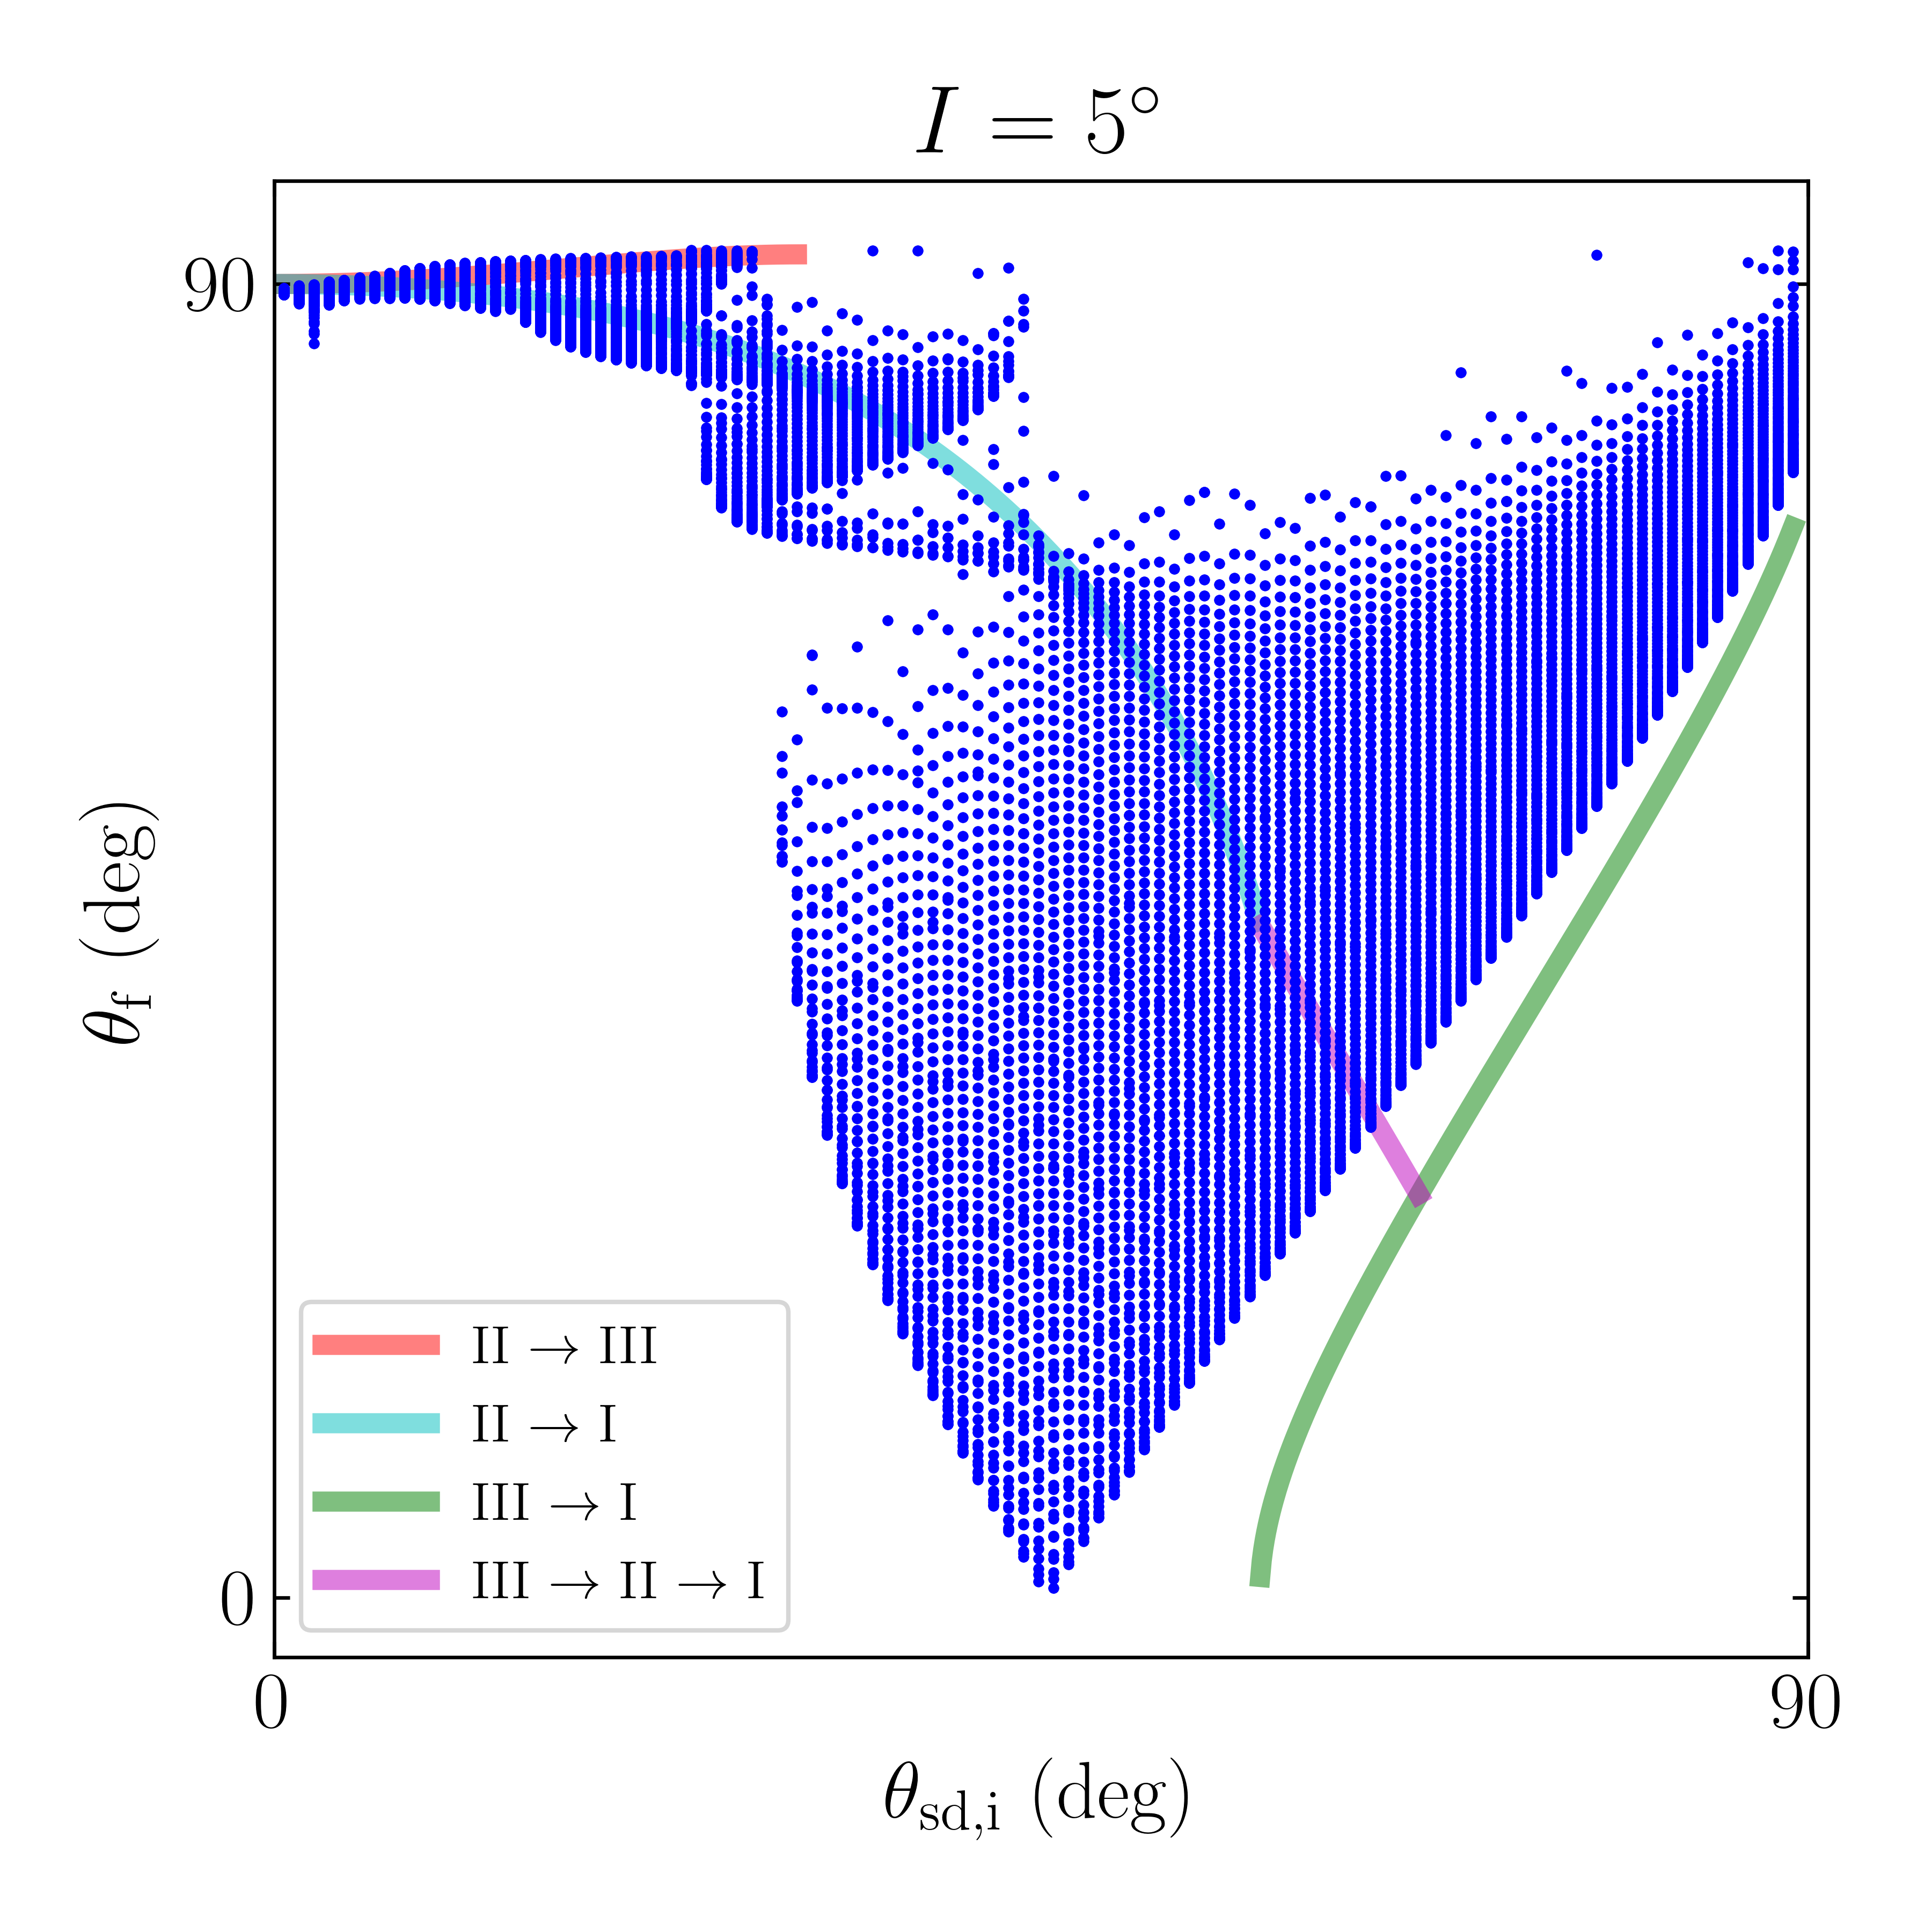
\includegraphics[width=0.8\textwidth]{../../initial/2_toy2/3_ensemble_05_15.png}
        \end{subfigure}
        \begin{subfigure}{0.45\textwidth}
            \centering
            \includegraphics[width=0.8\textwidth]{../../initial/2_toy2/3_ensemble_05_10.png}
        \end{subfigure}
    \end{figure}
\end{frame}

\begin{frame}
    \frametitle{Effect of Non-adiabaticity}
    \framesubtitle{Non-Adiabatic Fiducial Simulation}

    \begin{columns}
        \begin{column}{0.5\textwidth}
            \begin{figure}[t]
                \centering
                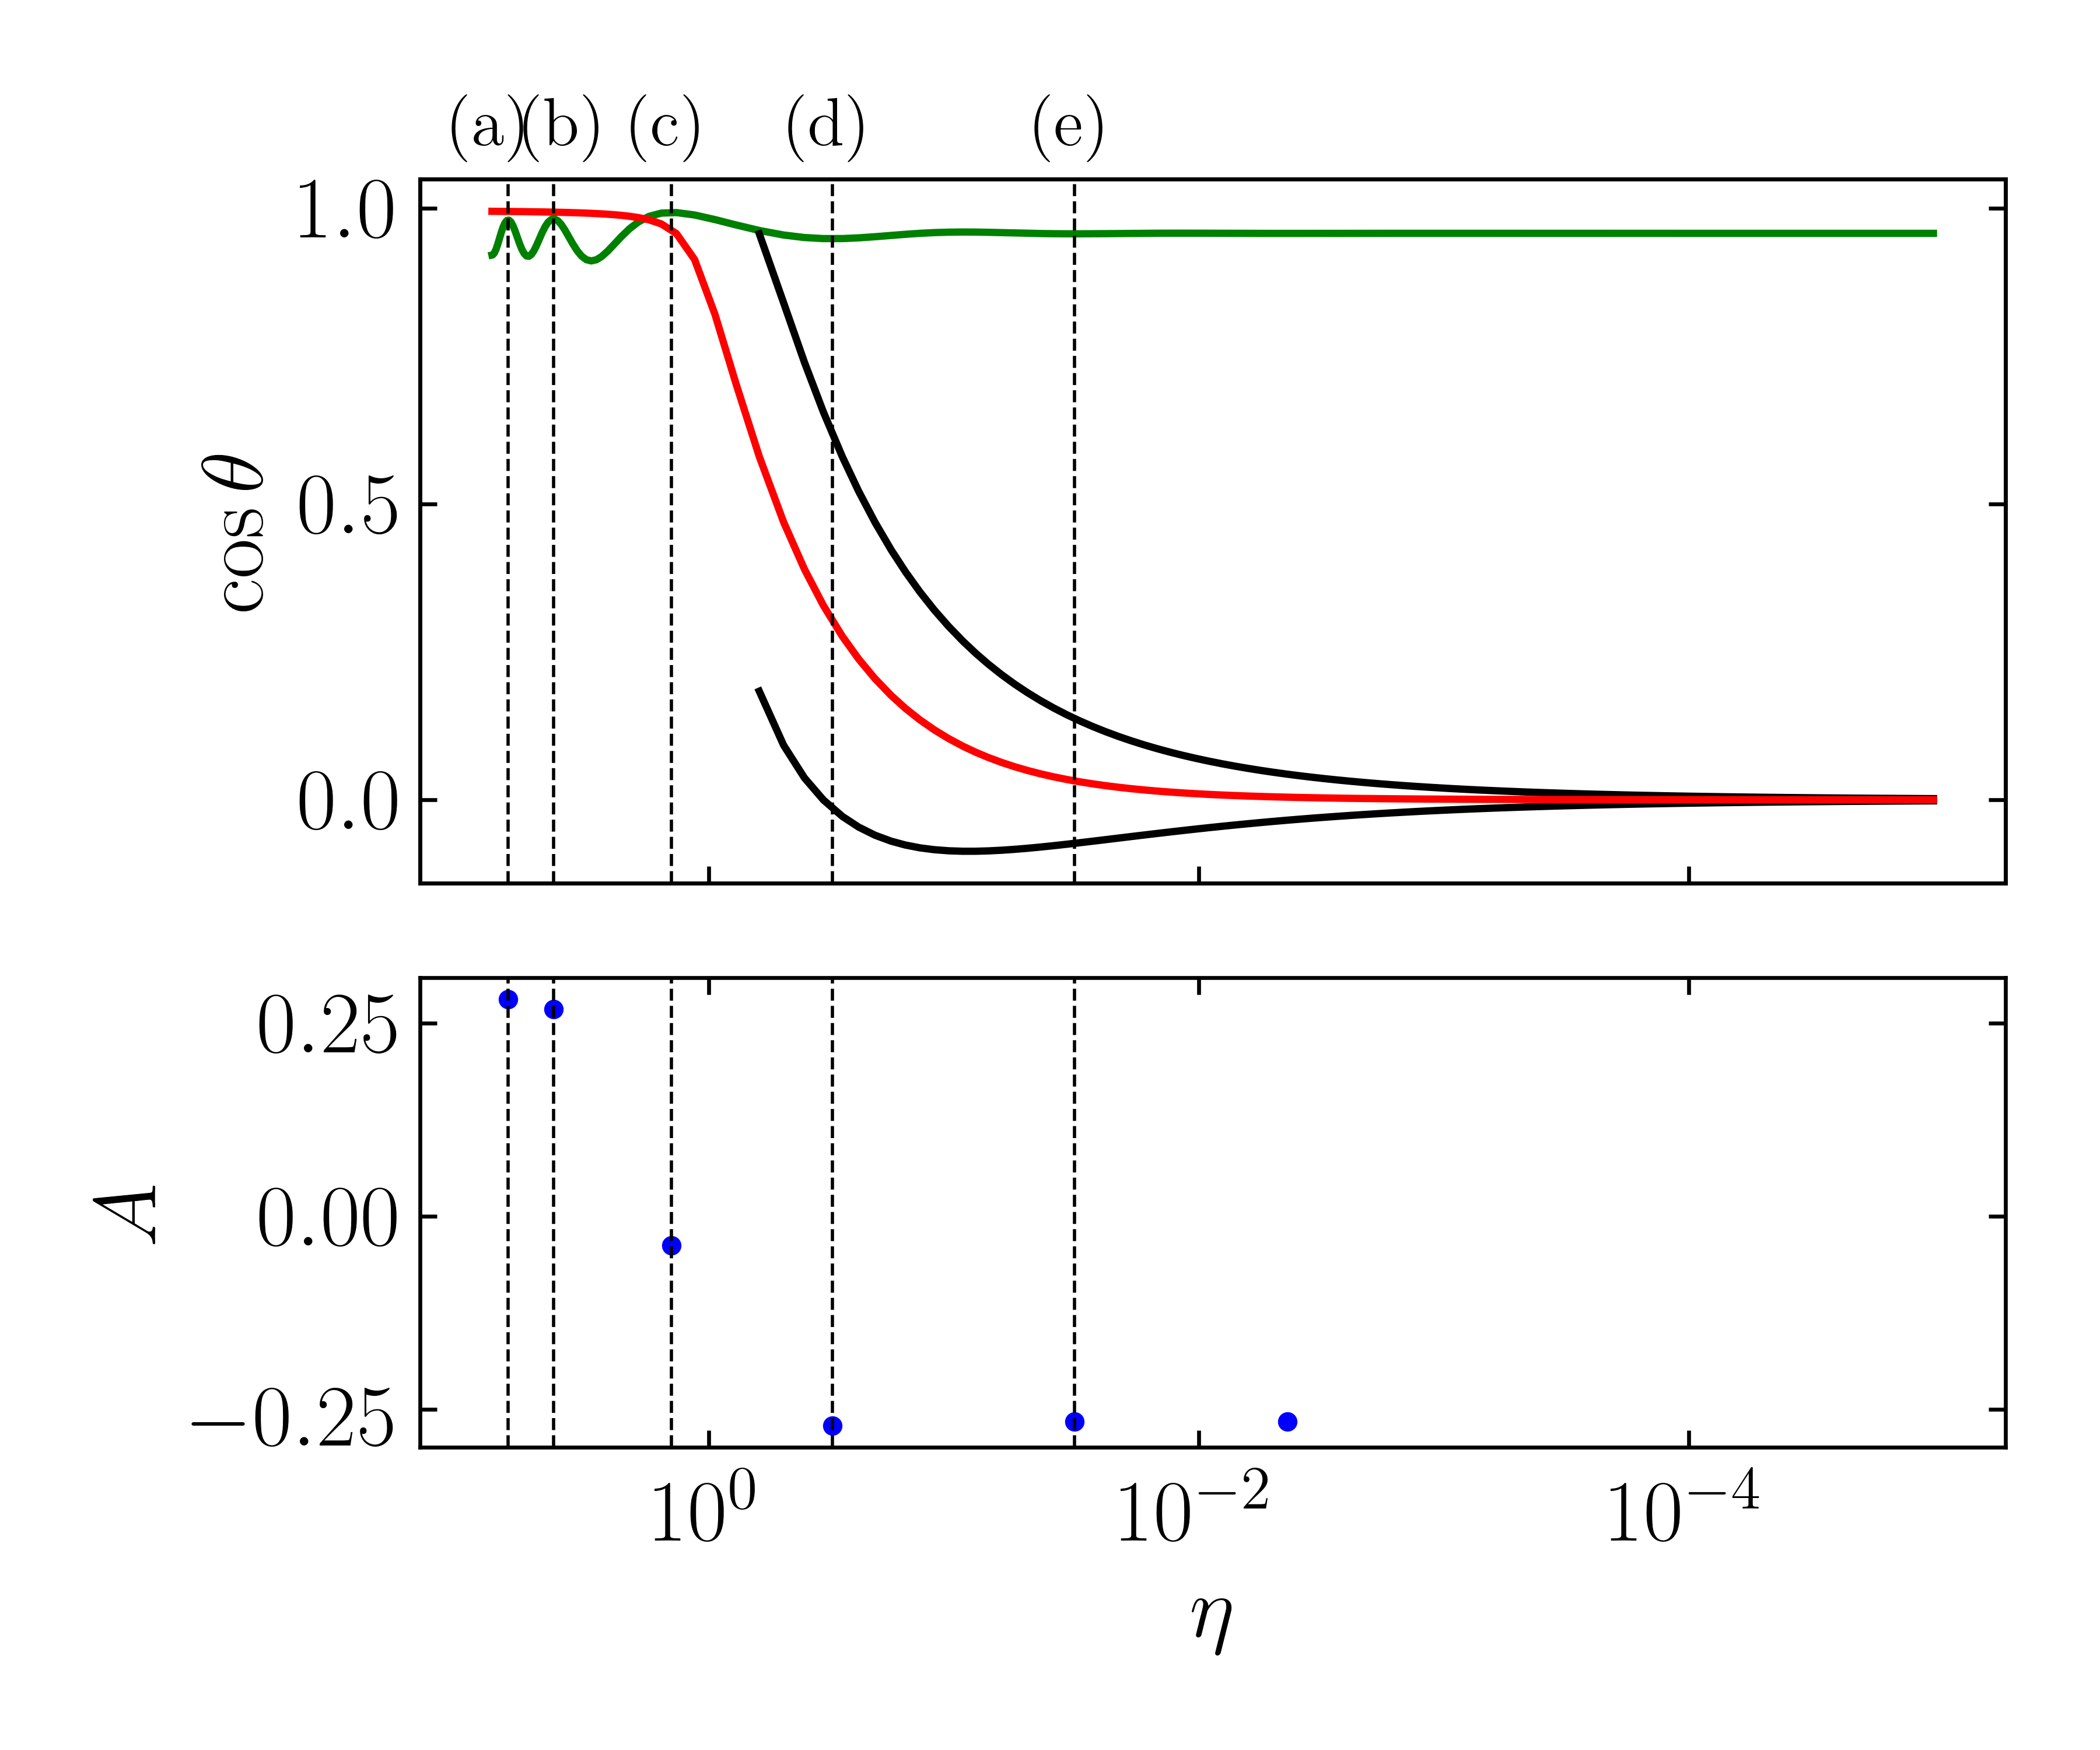
\includegraphics[width=\textwidth]{../../initial/2_toy2/3testo_nonad.png}
            \end{figure}
        \end{column}
        \begin{column}{0.5\textwidth}
            \begin{figure}[t]
                \centering
                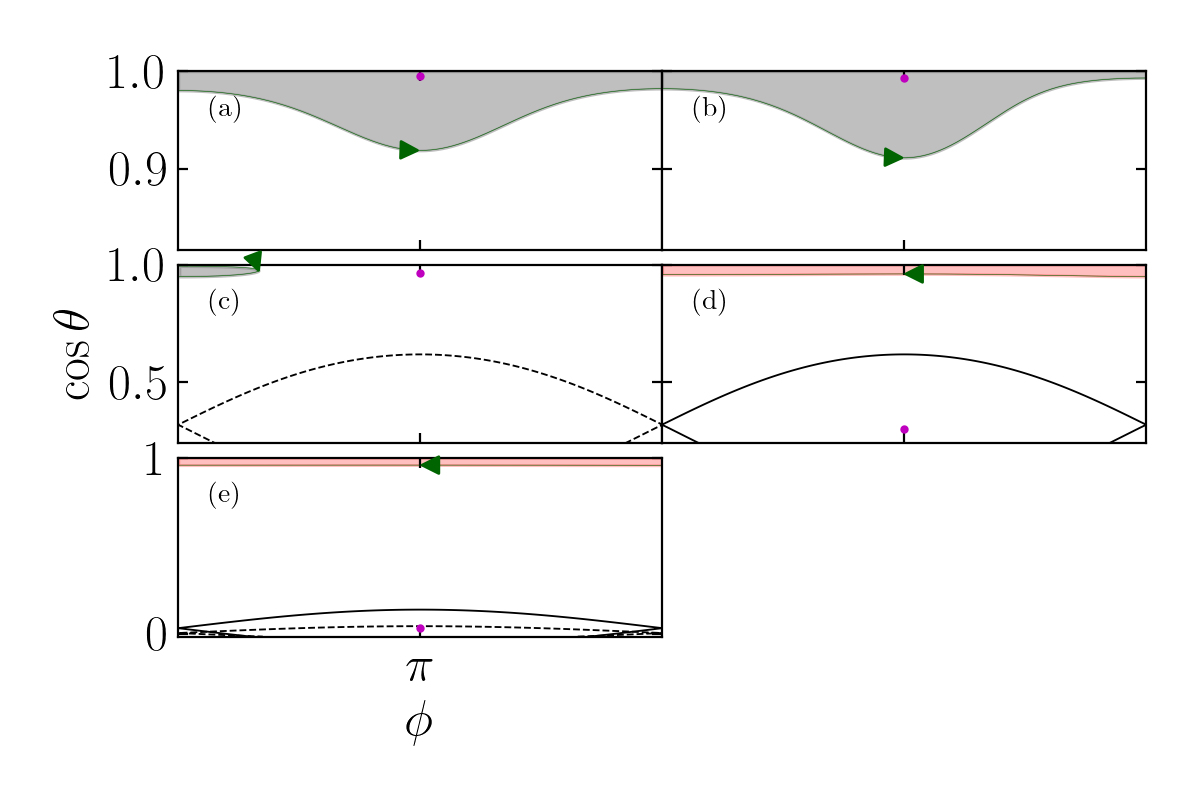
\includegraphics[width=\textwidth]{../../initial/2_toy2/3testo_nonad_subplots.png}
            \end{figure}
        \end{column}
    \end{columns}
\end{frame}

\begin{frame}
    \frametitle{Effect of Non-adiabaticity}
    \framesubtitle{Non-adiabatic Regime}
    \begin{columns}
        \begin{column}{0.5\textwidth}
            \begin{figure}[t]
                \centering
                \includegraphics[width=\textwidth]{../../initial/2_toy2/3_ensemble_05_06.png}
            \end{figure}
        \end{column}
        \begin{column}{0.5\textwidth}
            \begin{figure}[t]
                \centering
                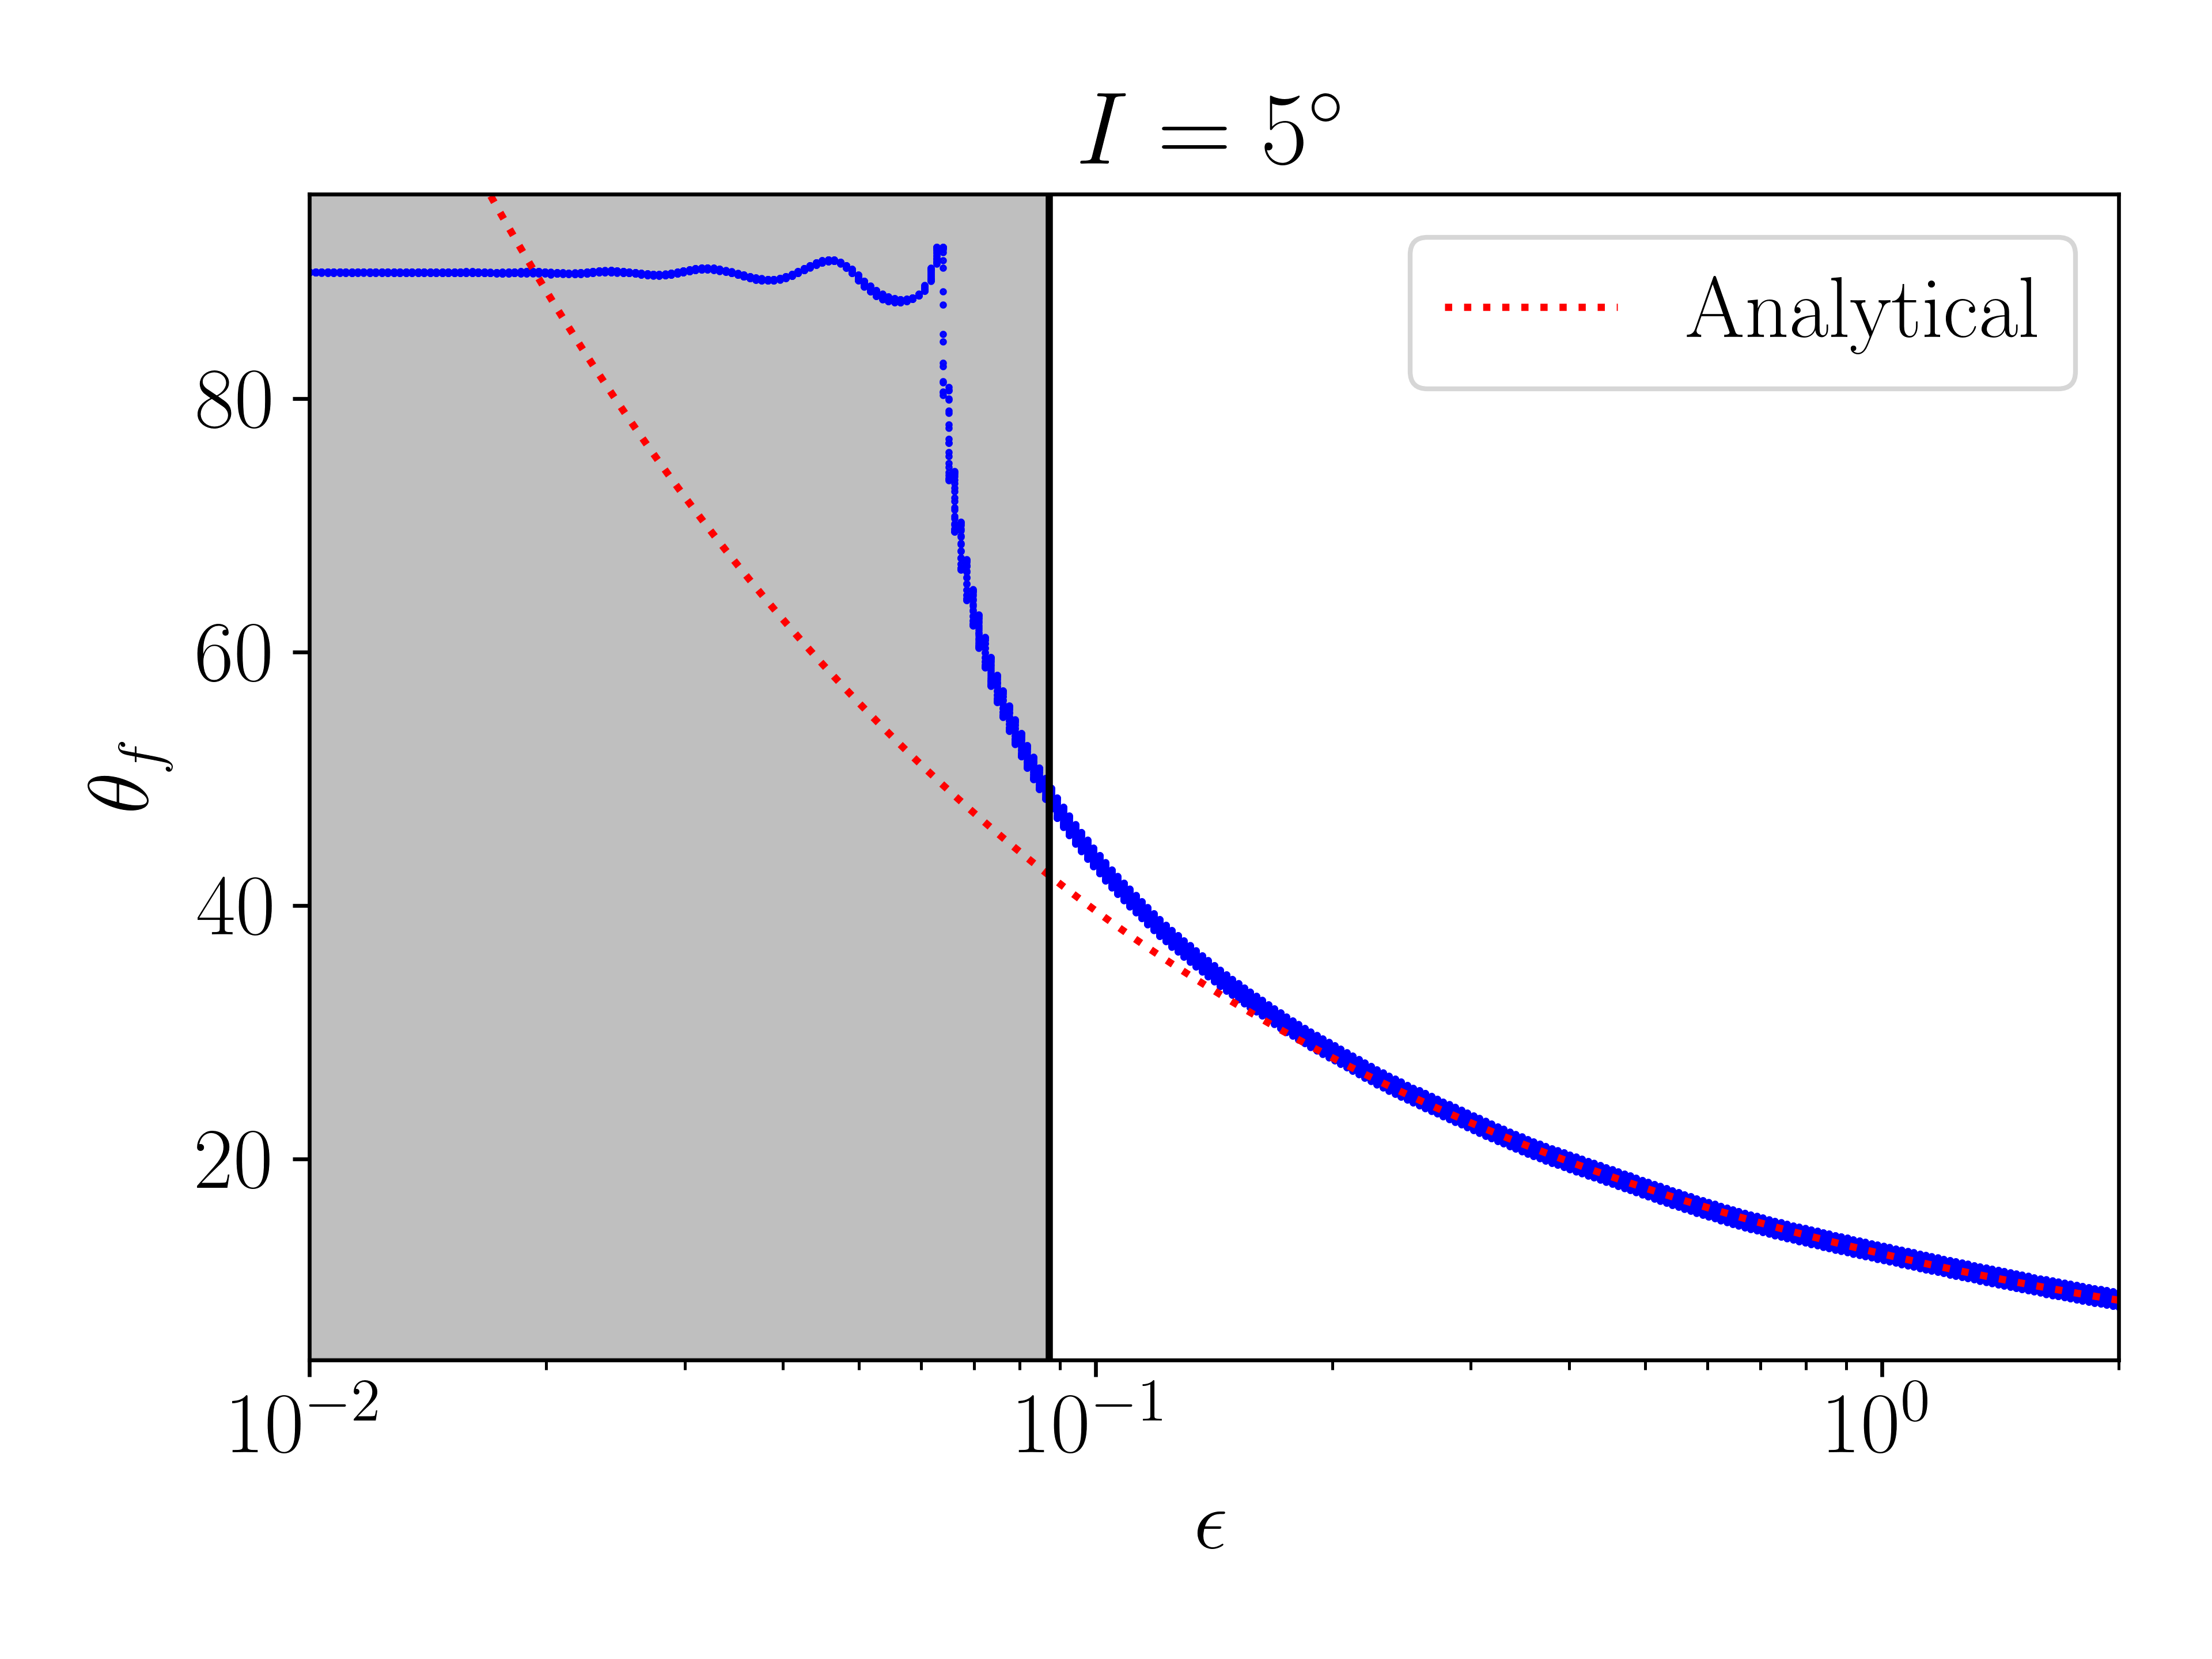
\includegraphics[width=\textwidth]{../../initial/2_toy2/3scan.png}
            \end{figure}
        \end{column}
    \end{columns}
\end{frame}

\begin{frame}
    \frametitle{Effect of Non-adiabaticity}
    \framesubtitle{Non-adiabatic Regime}
    \begin{columns}
        \begin{column}{0.5\textwidth}
            \begin{figure}[t]
                \centering
                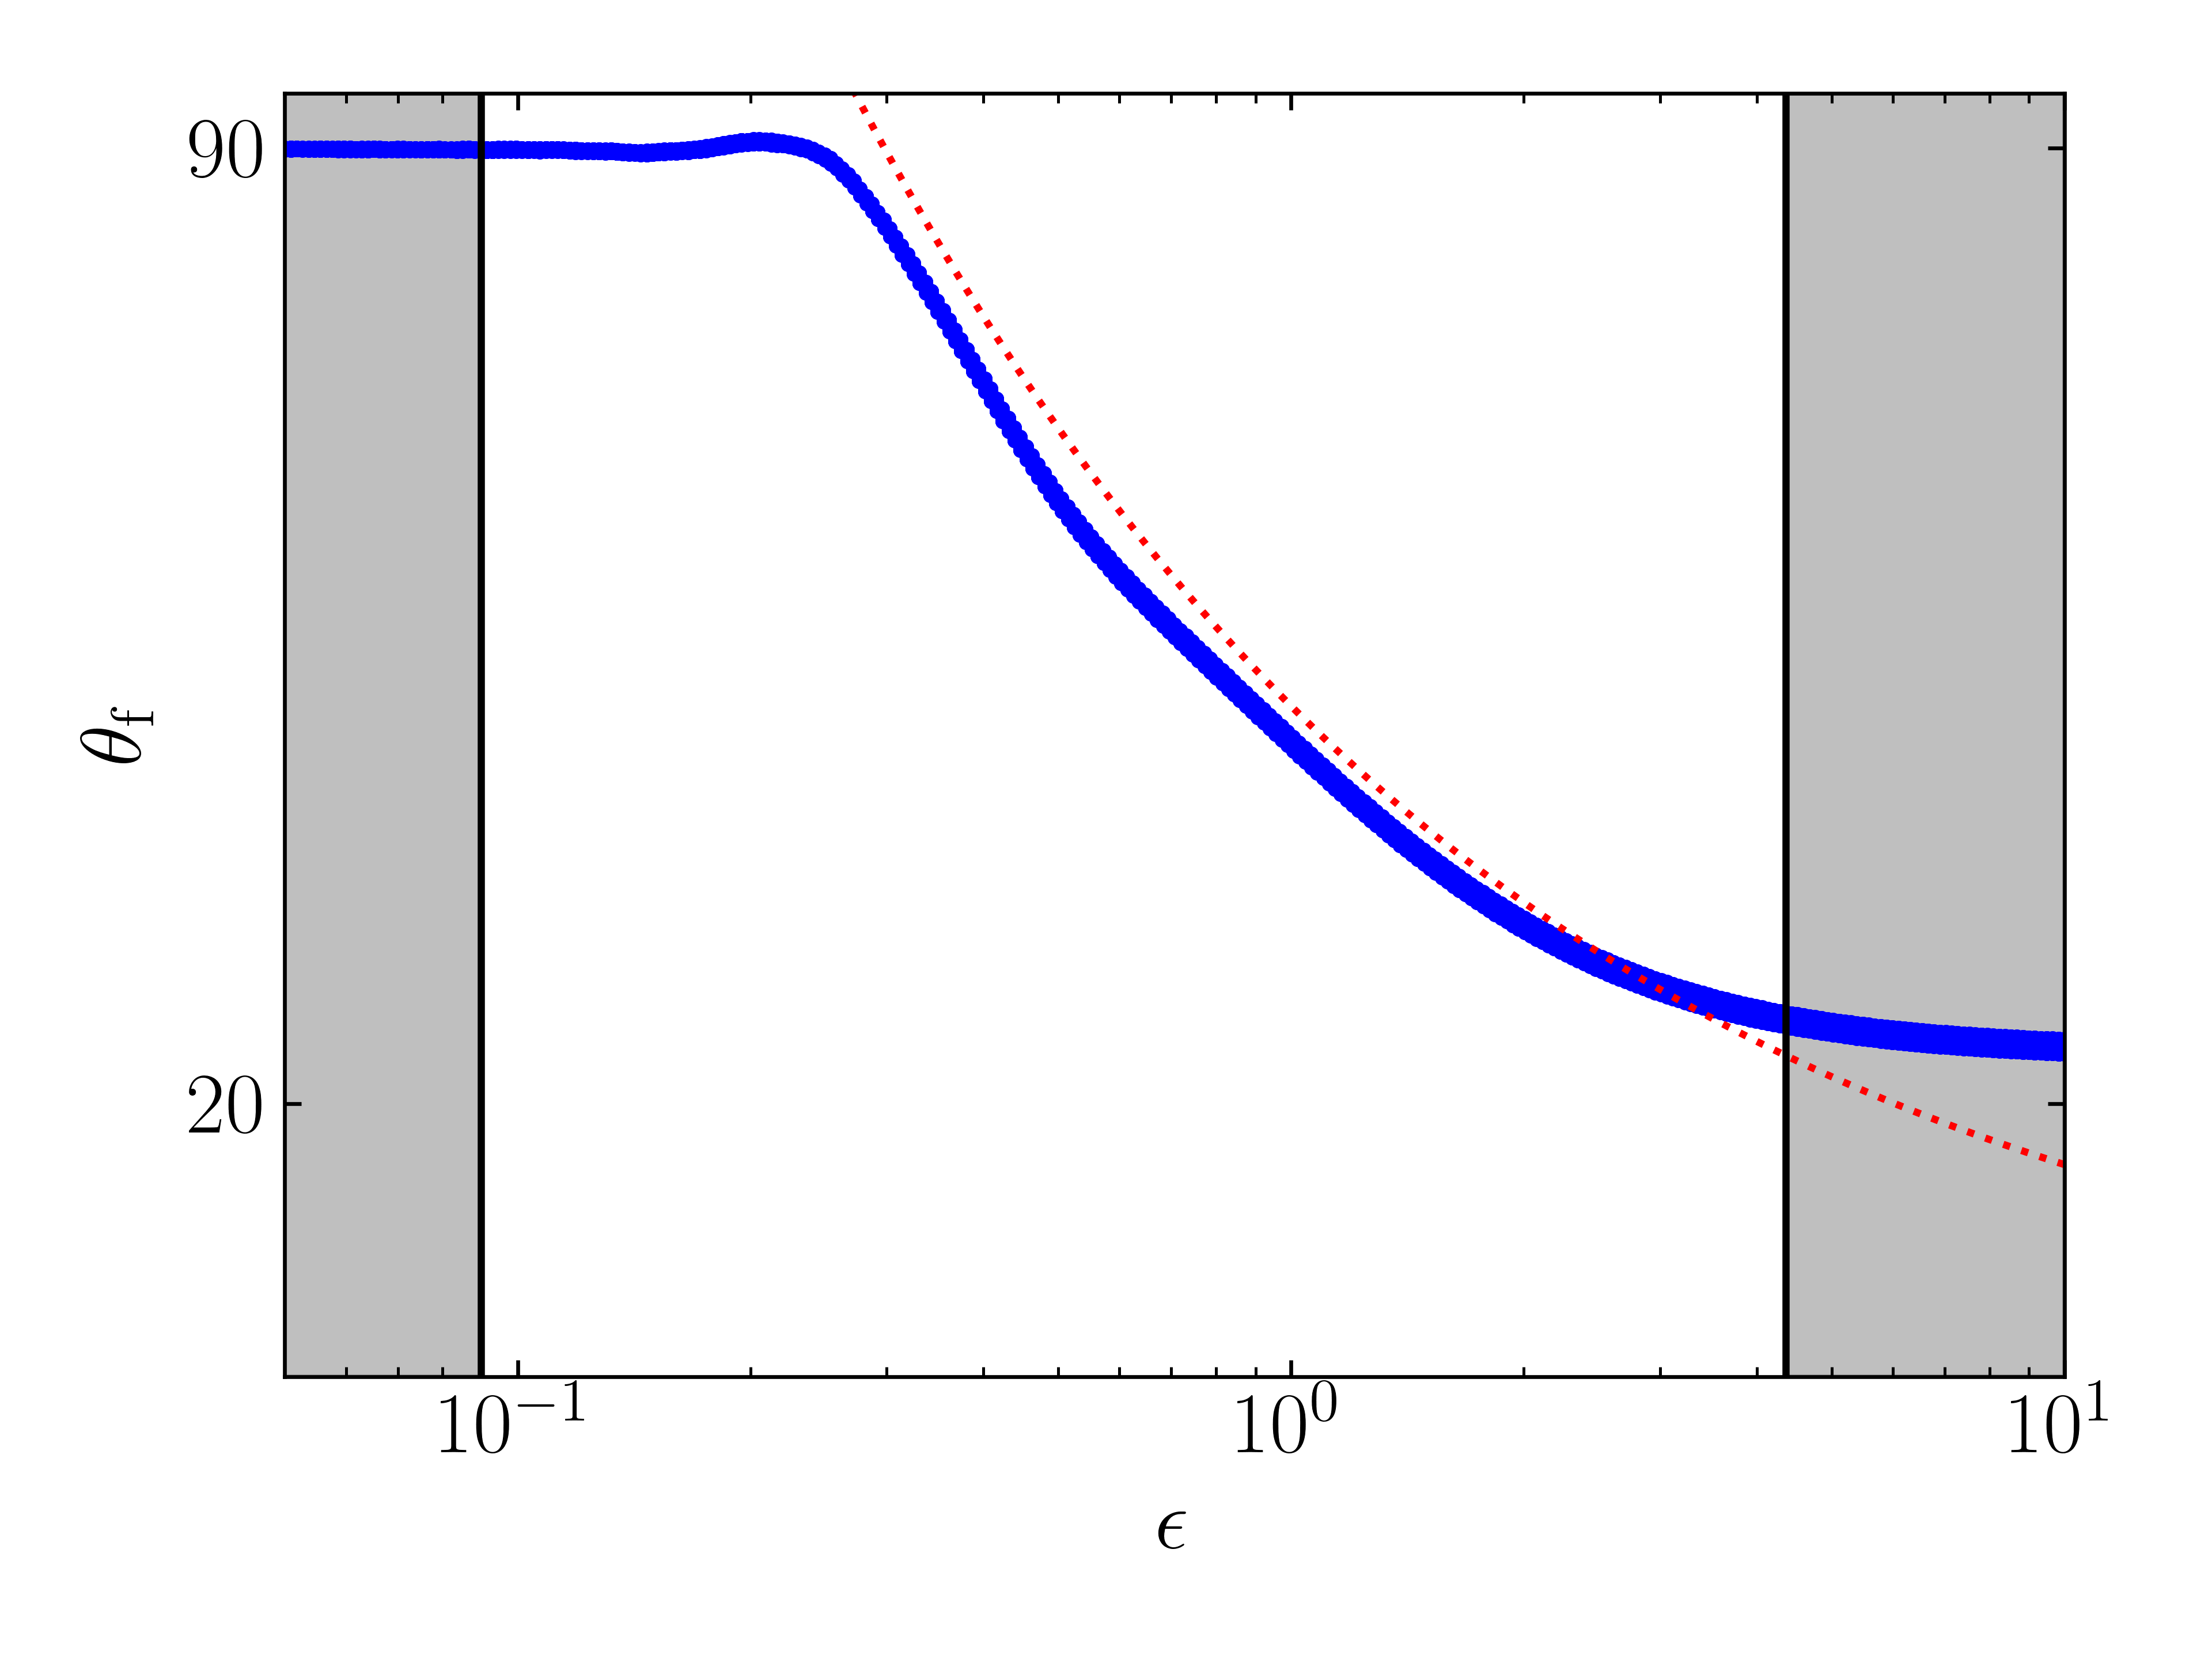
\includegraphics[width=\textwidth]{../../initial/2_toy2/3scan_20.png}
            \end{figure}
        \end{column}
        \begin{column}{0.5\textwidth}
            In the non-adiabatic regime:
            \begin{equation*}
                -\theta_{sd, i} \lesssim
                    \theta_{f} - \tan I \sqrt{\frac{2\pi}{\epsilon}} \lesssim
                    \theta_{sd, i}.
            \end{equation*}
        \end{column}
    \end{columns}
\end{frame}

\begin{frame}
    \frametitle{Future Work}

    \begin{itemize}
        \item Stability including dissipative perturbations (tides).
            \begin{itemize}
                \item At equilibrium: obliquity tides.
                \item During resonance advection.
            \end{itemize}

        \item Dynamics including dissipative perturbations.
            \begin{itemize}
                \item Weak tidal friction $\rd{\eta}{t}$, \textbf{new}
                    technique!
            \end{itemize}
    \end{itemize}
\end{frame}

\end{document}

